% !TEX program = pdflatex
% !TEX root = Bernal_H_JET.tex
\documentclass[review,authoryear,12pt]{elsarticle}
\usepackage[T1]{fontenc}
\usepackage{times}
\usepackage{amssymb,mathtools,amsthm}

\RequirePackage[colorlinks,citecolor=blue,linkcolor=blue,urlcolor=blue]{hyperref}
\RequirePackage{float}
\RequirePackage{graphicx}
\RequirePackage{subcaption}
\captionsetup[figure]{skip=6pt}
\captionsetup[subfigure]{font=footnotesize,aboveskip=3pt,belowskip=2pt}
\setlength{\abovecaptionskip}{6pt}
\setlength{\belowcaptionskip}{4pt}
\setlength{\intextsep}{10pt plus 2pt minus 2pt}
\setlength{\textfloatsep}{16pt plus 2pt minus 4pt}
\setlength{\floatsep}{12pt plus 2pt minus 2pt}
\newlength{\subfigheight}
\setlength{\subfigheight}{4.2cm}
\newlength{\mapfigheight}
\setlength{\mapfigheight}{4.55cm}
\newlength{\widefigheight}
\setlength{\widefigheight}{3.4cm}
\newlength{\calfigheight}
\setlength{\calfigheight}{3.2cm}
\newlength{\calbeliefheight}
\setlength{\calbeliefheight}{4.5cm}
\newlength{\calseriesheight}
\setlength{\calseriesheight}{3.8cm}
\newlength{\calplotheight}
\setlength{\calplotheight}{4.2cm}
\newlength{\calpathheight}
\setlength{\calpathheight}{5.1cm}
\newcommand{\panelgraphic}[2]{%
  \parbox[t][#1][t]{\linewidth}{\centering\includegraphics[width=\linewidth,height=#1,keepaspectratio]{#2}}%
}
\newcommand{\figurenote}[1]{%
  \par\vspace{3pt}%
  \begingroup\footnotesize #1\par\endgroup
}
\RequirePackage{amsmath,amssymb,mathtools}
\RequirePackage{booktabs}
\RequirePackage{longtable}
\RequirePackage{tabularx}
\RequirePackage{array}
\RequirePackage{etoolbox}
\providecommand{\textcite}{\citet}

\graphicspath{{./Figures/}}


\theoremstyle{plain}
\newtheorem{theorem}{Theorem}
\newtheorem{proposition}[theorem]{Proposition}
\newtheorem{lemma}[theorem]{Lemma}
\newtheorem{corollary}[theorem]{Corollary}

\theoremstyle{definition}
\newtheorem{definition}[theorem]{Definition}
\newtheorem{assumption}[theorem]{Assumption}
\newtheorem{remark}[theorem]{Remark}

\newenvironment{fnnote}{%
  \begin{minipage}[t]{\linewidth}%
  \sloppy
}{\end{minipage}}

\newcommand{\thmendmark}{\par\nobreak{\hfill\ensuremath{\square}\par}}
\AtEndEnvironment{theorem}{\thmendmark}
\AtEndEnvironment{proposition}{\thmendmark}
\AtEndEnvironment{lemma}{\thmendmark}
\AtEndEnvironment{corollary}{\thmendmark}
\AtEndEnvironment{definition}{\thmendmark}
\AtEndEnvironment{assumption}{\thmendmark}
\AtEndEnvironment{remark}{\thmendmark}

\newcommand{\E}{\mathbb{E}}
\newcommand{\Prob}{\mathbb{P}}
\newcommand{\ProbE}{\mathbb{P}_{\mathrm{E}}}
\newcommand{\ProbC}[1]{\mathbb{P}_{\mathrm{C},#1}}
\newcommand{\ThetaK}{\Theta_K}
\newcommand{\TV}{\mathrm{TV}}
\newcommand{\dd}{\mathrm{d}}
\newcommand{\1}{\mathbf{1}}
\newcommand{\argmin}{\operatorname*{arg\,min}}
\newcommand{\argmax}{\operatorname*{arg\,max}}
\newcommand{\supp}{\operatorname{supp}}
\newcommand{\Dirac}{\delta}
\newcommand{\ProbI}[1]{\mathbb{P}_{\mathrm{I},#1}}
\newcommand{\Unif}{\mathrm{Unif}}



\renewcommand{\thetable}{\Roman{table}}
\renewcommand{\thefigure}{\Roman{figure}}
\providecommand{\doi}[1]{\href{https://doi.org/#1}{doi:\detokenize{#1}}}

% Plain, unboxed title-page layout (no "Abstract" heading, no horizontal
% rules) to match the Bernal_H.tex (econsocart) front page.
\makeatletter
\abstracttitle{}
% Tighter abstract box (no empty heading/medskip, reduced line spacing) so the
% abstract + keywords/JEL block fits on a single page together with the title.
\renewenvironment{abstract}{\global\setbox\absbox=\vbox\bgroup
  \hsize=\textwidth
  \linespread{0.92}\selectfont
  \noindent\ignorespaces}
 {\egroup}
\long\def\pprintMaketitle{\clearpage
  \iflongmktitle\if@twocolumn\let\columnwidth=\textwidth\fi\fi
  \resetTitleCounters
  \def\baselinestretch{1}%
  \printFirstPageNotes
  \begin{\elsarticletitlealign}%
 \thispagestyle{pprintTitle}%
   \def\baselinestretch{1}%
    \Large\@title\par\vskip14pt%
    \ifdoubleblind
      \vspace*{2pc}
    \else
      \normalsize\elsauthors\par\vskip8pt
      \footnotesize\itshape\elsaddress\par\vskip14pt
    \fi
    \ifvoid\absbox\else\unvbox\absbox\par\vskip8pt\fi
    \ifvoid\keybox\else\unvbox\keybox\par\vskip8pt\fi
    \end{\elsarticletitlealign}%
    \gdef\thefootnote{\arabic{footnote}}%
  }
\makeatother

\begin{document}

\begin{frontmatter}

\title{Indirect Dynamic Mechanism Design with Endogenous Implementation Noise: Identifying Rational Types under Observational Pooling\tnoteref{t1}}
\tnotetext[t1]{Economist, professor of the economics program at the Universidad Colegio Mayor de Cundinamarca and Ph.D. in economics from the Universidad de los Andes, Colombia. E-mail: \href{mailto:hbernal@uniandes.edu.co}{hbernal@uniandes.edu.co}, \href{mailto:hbernalc@universidadmayor.edu.co}{hbernalc@universidadmayor.edu.co}. ORCID: \href{https://orcid.org/0000-0002-4864-1726}{0000-0002-4864-1726}. All research is the sole responsibility of the author, received no funding, and was developed as an independent initiative.}

\author{Humberto Bernal}

\address{Economics Program, Universidad Colegio Mayor de Cundinamarca; Ph.D. in Economics, Universidad de los Andes, Colombia.}

\begin{abstract}
This paper studies dynamic indirect mechanism design when a principal must screen an agent whose equilibrium actions pool, so passive observation cannot separate types. The contribution is theoretical. The paper introduces the Mano de Dios--Guadalupe (MDG) process, an endogenous-noise implementation kernel that maps latent strategic intentions into executed actions while preserving full support off the equilibrium path without an exogenous trembling-hand perturbation. Combining MDG with competing risks and an active information-acquisition motive, the paper establishes a Type Identification Theorem: uniform total-variation separation between type-contingent observation laws implies mutual singularity of trajectory laws by the criterion of \citet{Kakutani1948}, so Bayesian beliefs converge almost surely to the true type on the prolonged-interaction event. A Conditional Mechanism Implementability Theorem then guarantees a perfect Bayesian equilibrium satisfying incentive compatibility and individual rationality whenever the feasible policy set is non-empty. Both results are machine-checked in Lean~4. Kidnapping for ransom in Colombia is used as an applied validation: microeconometric fingerprints calibrate type-specific hazards, and ELN--PAR simulations illustrate finite-horizon learning, instrument paths, and constraint compliance under the calibrated mechanism.
\end{abstract}

\begin{keyword}
indirect mechanism design \sep dynamic screening \sep endogenous implementation noise \sep Bayesian learning \sep type identification \\
\textit{JEL classification:} C73 \sep D82 \sep D86
\end{keyword}

\end{frontmatter}

\section{Introduction and Related Literature}\label{sec:intro}

Mechanism design asks how a principal can implement an allocation when agents hold private information and act strategically. In the classical program of \citet{Gibbard1973} and \citet{Myerson1979IC,Myerson1981}, the Revelation Principle represents any incentive-compatible outcome of an indirect mechanism by an equivalent direct mechanism in which truthful reporting is optimal. That representation is a theoretical reduction, not an institutional prescription: when messages are restricted, actions are noisy, or types refuse literal revelation, the economically relevant object remains an \emph{indirect} mechanism based on observable actions, public histories, and implementable instruments \citep{Jackson2001,BergemannMorris2012}. The present paper develops such an object for dynamic environments in which equilibrium behavior pools: distinct types generate observationally similar short-run signals, so a myopic policy that minimizes current loss can freeze the very pooling that prevents identification tomorrow.

The central design problem is therefore threefold. First, how should the principal specify an action-based indirect mechanism when the message space is not a free report of type? Second, how can implementation frictions be modeled endogenously so that Bayes' rule remains well defined off path, without relying on an exogenous trembling-hand device? Third, under what conditions do public signals identify the agent's true type, and when is the resulting policy rule implementable in perfect Bayesian equilibrium (PBE)? The paper is situated at the frontier of dynamic mechanism design, expanding the foundational theoretical frameworks of \citet{CourtyLi2000}, \citet{EsoSzentes2007}, and \citet{PavanSegalToikka2014} by incorporating active informational exploration and structural noise, which are indispensable for its viability in adversarial institutional contexts.

\subsection{Contribution relative to the literature on indirect mechanisms}\label{subsec:framing}

Relative to the static implementability frontier defined by \citet{MyersonSatterthwaite1983}, \citet{Rochet1987}, and \citet{RochetChone1998}, and complementing the general existence conditions established by \citet{KadanRenySwinkels2017}, the central contribution of this work lies in formulating and characterizing an indirect dynamic mechanism subject to endogenous implementation noise. This approach introduces an intrinsic stochastic friction between the agent's latent strategic intention and the publicly recorded action, enabling both the Bayesian identification of rational types and conditional implementability under the perfect Bayesian equilibrium (PBE) criterion. Specifically, the paper structures this contribution through four interconnected theoretical results.

\paragraph{Indirect action-based dynamic mechanism.}
The paper formalizes a dynamic indirect mechanism in which the principal chooses instruments as functions of public history and beliefs, while private agents best-respond in their information sets. Types need not be reported; they are inferred from the law of executed actions and outcomes. This preserves the Revelation Principle as a representation theorem while insisting that, for the environments considered here, the operational design object is the indirect rule.

\paragraph{MDG endogenous implementation kernel.}
The Mano de Dios--Guadalupe (MDG) process---equivalently, an endogenous implementation kernel---maps latent intentions $a_t^{i\ast}$ into executed actions $\tilde a_t^i$ through a hybrid-temperature logit with full support. Unlike classical refinements that inject exogenous trembles into strategies \citep{Selten1975Perfectness,KrepsWilson1982}, MDG treats implementation noise as an intrinsic friction of materialization. Under a positive residual floor, the kernel maintains absolute continuity in the sense of \citet{KalaiLehrer1993}, keeping Bayesian updating well defined on every branch while concentrating mass on the intended action. A maximum-entropy characterization in the spirit of \citet{Jaynes1957Information} disciplines the functional form.

\paragraph{Type Identification Theorem for rational types.}
When each type induces a structural fingerprint that separates daily observation laws uniformly in total variation, the product-measure criterion of \citet{Kakutani1948} yields mutual singularity of trajectory laws. Combined with the martingale stability of beliefs \citep{Doob1953Stochastic,BlackwellDubins1962}, posterior mass concentrates almost surely on the true type on the prolonged-interaction event $\mathcal{T}=\{\tau=\infty\}$. The theorem converts a local daily separation condition into global identification. Its limitation is explicit: asymptotic consistency is stated on $\mathcal{T}$; finite-horizon simulations in the application illustrate directional learning without substituting for the asymptotic result.

\paragraph{Conditional PBE implementability.}
Identification alone does not make a mechanism executable. The Conditional Mechanism Implementability Theorem shows that, whenever the feasible set defined by incentive compatibility and individual rationality remains non-empty, there exists a PBE in which the principal's optimal rule implements the social choice subject to those constraints. Thus MDG, learning, and incentive feasibility form a single architecture: noise enables off-path updating; separation enables identification; and non-empty $\Gamma_t(\mu_t)$ enables equilibrium implementation.

\paragraph{Applied validation.}
Sections~\ref{sec:application}--\ref{sec:calibracion} map the abstract environment to kidnapping for ransom in Colombia. Multinomial logit and competing-risks estimates from National Center for Historical Memory microdata supply type-specific hazards; ELN and PAR calibrations then report posterior paths, instrument trajectories, informational gain, and IR/IC compliance. The application is a validation layer, not the theoretical primitive.

The remainder of the article proceeds as follows. Section~\ref{sec:model} presents the general indirect mechanism, the MDG kernel, competing risks, and best responses for arbitrary unknown types. Section~\ref{subsec:formal-defs} states the Type Identification Theorem. Section~\ref{sec:implementabilidad} establishes conditional PBE implementability and policy implications. Section~\ref{sec:application} specializes the environment to Colombian kidnapping and anchors parameters empirically. Section~\ref{sec:calibracion} reports calibration and simulations. Section~\ref{sec:conclusiones} concludes. Supplemental Appendices contain microeconometric detail and Lean~4 proofs.


\section{General Environment and Indirect Mechanism}\label{sec:model}

This section develops the theoretical model in general form. A principal designs an indirect dynamic mechanism when an agent's private type is unknown and equilibrium actions may pool. Types need not be elicited by direct reports: the mechanism operates on public histories, executed actions, and instruments. The Revelation Principle of \citet{Gibbard1973} and \citet{Myerson1979IC,Myerson1981} continues to imply that any incentive-compatible indirect outcome admits a direct representation; the contribution here is to construct and analyze the indirect object itself when messages are restricted to materialized actions subject to endogenous implementation noise. Kidnapping for ransom appears only later (Section~\ref{sec:application}) as a concrete specialization of the same primitives.

\paragraph{Primitives (general notation).}
Let $\mathcal{J}$ be a finite set of players containing a principal $P$ and privately informed agents. Each episode is indexed by discrete time $t\in\mathbb{T}$ until an endogenous stopping time $\tau$. A type $\theta\in\Theta$ is drawn from a common prior $\mu_0\in\Delta(\Theta)$ with full support; only a designated agent observes the strategically relevant component of $\theta$. In each period the principal chooses instruments $x_t$ as a measurable function of public history $h_t$ and beliefs $\mu_t$; agents choose latent intentions $a_t^{i\ast}$; an implementation kernel $Q_t(\tilde a_t^i\mid a_t^{i\ast},x_t,h_t)$---the MDG process---delivers executed actions $\tilde a_t^i$; public signals $\zeta_t$ update $\mu_{t+1}$ by Bayes' rule. The design goal is to implement a social choice rule that is sequentially rational, incentive compatible, and individually rational while inducing informative laws of observation.

\paragraph{Specialization used below.}
For concreteness and continuity with the Lean-checked theorems, the remainder of this section writes the general objects in the language of a three-player adversarial screening game $\{S,K,F\}$ (principal, informed adversary, and complementary agent), with private type $\theta_K\in\ThetaK$, instruments $(\alpha_t,\gamma_t)$, and competing-risk outcomes. Nothing in the identification or implementability arguments requires the labels ``state,'' ``captor,'' or ``family'': those names are interpretive. The Colombian type menu $\{\mathrm{DC},\mathrm{PAR},\mathrm{ELN},\mathrm{FARC}\}$ is introduced only when the application maps $\ThetaK$ to estimated criminal technologies.

\subsection{Definition of the mechanism}\label{subsec:def-mecanismo}


Let $\mathcal{J}=\{S,K,F\}$ be the set of players in the specialized notation, where $S$ is the principal (state), $K$ the privately informed agent (adversary), and $F$ a complementary agent (family). Each episode is characterized by the vector of types $\theta=(\theta_K,\theta_F,\theta_V,\theta_S)\in\Theta$, where the strategically private component $\theta_K$ takes values in a finite menu $\ThetaK$. In the Colombian application of Section~\ref{sec:application}, $\ThetaK=\{\text{DC},\text{PAR},\text{ELN},\text{FARC}\}$ indexes distinct criminal technologies---common delinquency, paramilitary groups, National Liberation Army, and Revolutionary Armed Forces of Colombia---but the theorems treat $\ThetaK$ as an arbitrary finite type space; $\Theta_F=\{\text{High},\text{Low}\}$ represents the family's payment capacity; $\Theta_V=\{\text{Public},\text{Private}\}$ represents the victim's profile; and $\Theta_S=\{\text{Hard},\text{Lax}\}$ represents the institutional environment. Each episode is also localized in an observable geographic zone $z\in\mathcal{R}$, where $\mathcal{R}$ groups five regions (Metropolitan, Andean, Caribbean, Pacific, and East-Jungle); $z$ is not a private strategic type but a public initial condition that disciplines the prior over the captor's type. Only $\theta_K$ is private information of $K$; the other components and $z$ are observable upon opening the episode, with an initial belief $\mu_0(\theta\mid z,\theta_V)=\Prob(\theta_K=\theta\mid z,\theta_V)\in\Delta(\ThetaK)$.


The public history $h_t\in H_t$ recursively records, up to the beginning of $t$ and without including the type vector $\theta$ or the belief $\mu_t$, the following elements: $t$ is the period index; $\alpha^\ast_{[0,t-1]}$ and $\gamma^\ast_{[0,t-1]}$ are the trajectories of the state's financial interdiction and operational pressure instruments; $\tilde{a}^F_{[0,t-1]}$, $\tilde{a}^K_{[0,t-1]}$, and $\tilde{a}^S_{[0,t-1]}$ are the actions executed by the family, the captor, and the state; $m_{[0,t-1]}$ is the sequence of physical outcomes; and $d_{[0,t-1]}$ is the sequence of institutional detection signals, where $d_t\in\{0,1\}$ indicates whether in period $t$ the state detected collusion between the family and the captor, i.e., a clandestine ransom payment bypassing the financial interdiction policy.
\begin{gather}
h_t = \bigl(t,\,\alpha^\ast_{[0,t-1]},\,\gamma^\ast_{[0,t-1]},\,\tilde{a}^F_{[0,t-1]},\,\tilde{a}^K_{[0,t-1]},\,\tilde{a}^S_{[0,t-1]},\,m_{[0,t-1]},\,d_{[0,t-1]}\bigr),\label{eq:historia-publica}\\
h_{t+1} = \bigl(h_t,\,\alpha_t^\ast,\,\gamma_t^\ast,\,\tilde{a}_t^F,\,\tilde{a}_t^K,\,\tilde{a}_t^S,\,m_t,\,d_t\bigr).\label{eq:actualizacion-historia}
\end{gather}
The information sets when choosing in $t$ are
\begin{gather*}
\mathcal{I}_t^S=\bigl(h_t,z,\theta_F,\theta_V,\theta_S,\mu_t\bigr),\\
\mathcal{I}_t^F=\bigl(h_t,z,\theta_F,\theta_V,\theta_S\bigr),\qquad
\mathcal{I}_t^K=\bigl(h_t,z,\theta_K,\theta_F,\theta_V,\theta_S\bigr).
\end{gather*}
Although $\mu_t$ is internal to the state, its exclusion from the private information sets does not generate inconsistency: in the PBE, private agents share the same prior and the same public history $h_t$, and therefore replicate the Bayesian updating of the planner \citet{FudenbergTirole1991}.

The space of institutional allocations of the state is $\mathcal{X}_t=\mathcal{A}^{S,\mathrm{disc}}\times\mathcal{A}^{\alpha}\times\mathcal{A}^{\gamma}$. In each period $t$, players formulate optimal strategic intentions $a_t^{i\ast}$; the MDG process transforms them into executed actions $\tilde{A}_t=(\tilde{a}_t^F,\tilde{a}_t^K,\tilde{a}_t^S)$ that enter the public registry and determine $h_{t+1}$ and the public signal $\zeta_t$. Conditional on the executed actions and the optimal institutional policy, the system determines the physical outcome $m_t\in\mathcal{M}_{\mathrm{out}}$ through a block of competing risks, with $\mathcal{M}_{\mathrm{cont}}=\{\mathrm{cont}\}$, where $\mathrm{cont}$ denotes the continuation of captivity, $\mathcal{M}_{\mathrm{term}}=\{\mathrm{pay},\mathrm{res},\mathrm{rel},\mathrm{kill}\}$, which groups the termination causes: ransom payment, tactical rescue, voluntary release, and death of the victim, respectively, and $\mathcal{M}_{\mathrm{out}}=\mathcal{M}_{\mathrm{cont}}\cup\mathcal{M}_{\mathrm{term}}$.

The horizon of the episode is not fixed in advance but is determined by the captivity dynamics themselves: the episode concludes in the first period in which a terminal outcome materializes, so the effective horizon is the endogenous stopping time
\begin{equation}
\tau=\inf\{t\geq 0:m_t\in\mathcal{M}_{\mathrm{term}}\},\label{eq:stopping-time}
\end{equation}
where the recursive construction of $h_t$ ensures that the event $\{\tau=t\}$ is measurable with respect to the public history at the beginning of $t$, guaranteeing that the state recognizes the closure of the episode in real time. On these elements, with $\mathbb{T}=\{0,1,\ldots,\tau\}$ as the active periods index, $\Theta=\ThetaK\times\Theta_F\times\Theta_V\times\Theta_S$ the type space, $(H_t)_{t\in\mathbb{T}}$ the family of public history spaces recursively generated by~\eqref{eq:historia-publica}--\eqref{eq:actualizacion-historia}, $(\mu_t)_{t\in\mathbb{T}}$ the belief process in $\Delta(\ThetaK)$ updated by Bayes' rule throughout the episode, and $\Prob$ the ex-ante law induced by the strategy profile $s$, the prior $\mu_0$, and the captivity dynamics, the dynamic indirect mechanism is formally defined as the tuple
\[
\mathcal{D}=\bigl\langle\mathcal{J},\,\mathbb{T},\,\Theta,\,\mathcal{R},\,(\mathcal{X}_t)_{t\in\mathbb{T}},\,(H_t)_{t\in\mathbb{T}},\,(\mu_t)_{t\in\mathbb{T}},\,\Prob\bigr\rangle.
\]
Given $z\in\mathcal{R}$ and $\theta_K\sim\mu_0$, the principal's strategy $s^S=\chi=(\chi_t)_{t\in\mathbb{T}}$ is implemented via the measurable public policy rule $\chi_t\colon H_t\times\mathcal{R}\to\mathcal{A}^{S,\mathrm{disc}}\times\mathcal{A}^{\alpha}\times\mathcal{A}^{\gamma}$, which interacts with the private responses of $K$ and $F$ in their information sets; the social choice rule is formalized by the measurable mapping $f_t\colon\mathcal{I}_t^S\to\mathcal{X}_t$, such that the policy vector in equilibrium is $x_t^\ast:=f_t(\mathcal{I}_t^S)=(a_t^{S\ast},\alpha_t^\ast,\gamma_t^\ast)\in\mathcal{X}_t$. This rule is implementable if it constitutes the path of a PBE in the sense of \citet{FudenbergTirole1991}, which guarantees that the informed agent cannot systematically induce the principal to calibrate instruments on a type that is not the true one; implementability is achieved when the pair $(s,\mu)$, with $s=(s^S,s^K,s^F)$ and $\mu_t\in\Delta(\ThetaK)$, satisfies two conditions in every reachable information set: \emph{sequential rationality}, whereby each agent $i\in\{K,F\}$ maximises $\mathcal{U}_t^i$ given $\mathcal{I}_t^i$ and the strategies of the others while the state minimizes the expected social loss weighted by $\mu_t$; and \emph{Bayesian consistency}, whereby in every node reached with positive probability under $\Prob^s$, the beliefs satisfy
\[
\mu_t(\theta)=\Prob^s\!\bigl(\theta_K=\theta\mid\mathcal{F}_t^{\mathrm{pub}}\bigr),\qquad \mathcal{F}_t^{\mathrm{pub}}=\sigma\bigl(z,\zeta_0,\ldots,\zeta_{t-1}\bigr),
\]
where $\mathcal{F}_t^{\mathrm{pub}}$ is the public filtration at the beginning of $t$, generated by the $\sigma$-algebra of the initial geographic location $z$ and the public signals $\zeta_0,\ldots,\zeta_{t-1}$; each signal $\zeta_u=(\alpha_u^\ast,\gamma_u^\ast,\tilde{a}_u^F,\tilde{a}_u^K,\tilde{a}_u^S,m_u,d_u)$ aggregates all observables of period $u$ and constitutes the informational support over which the state updates its beliefs about $\theta_K$; so that the instruments $(\alpha_t^\ast,\gamma_t^\ast)$ are calibrated on correct inferences about the captor's type.

\subsection{Summary of the mechanism}\label{subsec:resumen-mecanismo}

In each active period $t$, the protocol advances in three sequential stages. In the first, the agents formulate their optimal intentions: the state resolves $x_t^\ast=f_t(\mathcal{I}_t^S)$, and private agents select their best responses in their respective information sets, conditioned on the observable public policy $(\alpha_t^\ast,\gamma_t^\ast)$ signaled by the state. In the second, the MDG process transforms these intentions into executed actions $\tilde{A}_t$, guaranteeing full support across all branches of the game. In the third, the material state of the episode
\[
\mathcal{C}_t(\theta_K)=\bigl(\theta_K,\theta_F,\theta_V,\theta_S,z,\tilde{a}_t^F,\tilde{a}_t^K,\tilde{a}_t^S,\alpha_t^\ast,\gamma_t^\ast,p_{\mathrm{det},t}\bigr),
\]
with $p_{\mathrm{det},t}$ as the logit probability of detecting collusion, which is increasing in the state's instruments. This material state feeds a block of competing risks that determines $m_t$ and $d_t$; the public signal $\zeta_t$ aggregates all observables of the period and updates the history to $h_{t+1}$ and the belief to $\mu_{t+1}$ through Bayes' rule.

\subsection{Probabilistic technology}\label{subsec:prob-tech}

This section formalizes the stochastic architecture that transforms strategic plans into observable realizations. In the base specification, the MDG process takes as input the latent strategic intention $a_t^{i\ast}$ and generates an executed action $\tilde{a}_t^i$ through an implementation law concentrated on the plan, but with full support over $\mathcal{A}^i$. The executed profile $\tilde{A}_t=(\tilde{a}_t^K,\tilde{a}_t^S,\tilde{a}_t^F)$ is the observable variable that enters the public record, while the strategic intention remains latent. Given $a_t^{i\ast}\in\mathcal{A}^i$ and the state vector $X_t$, execution is determined by
\[
\tilde{a}_t^i\sim\ProbI{i}\bigl(\tilde{a}_t^i\mid a_t^{i\ast},X_t\bigr),
\]
and, for each agent $i\in\{K,S,F\}$ and action $a\in\mathcal{A}^i$, it is specified as
\begin{equation}
\ProbI{i}\bigl(\tilde{a}_t^i=a\mid a_t^{i\ast},X_t\bigr)
=\frac{\exp\bigl(\mathbf{1}\{a=a_t^{i\ast}\}/T_t\bigr)}{\sum_{a'\in\mathcal{A}^i}\exp\bigl(\mathbf{1}\{a'=a_t^{i\ast}\}/T_t\bigr)},
\label{eq:mdg}
\end{equation}
where $T_t>0$ in the base specification is the temperature of the system: it measures the implementation friction of the episode, not the agent's uncertainty about its own type. To capture strategic learning and institutional maturation jointly, define
\begin{equation}
T_t=T_0\max\Bigl\{\frac{H(\mu_t)}{H(\mu_0)}e^{-\eta_{\mathrm{cal}}t},\,\underline{c}\Bigr\},
\label{eq:temperature}
\end{equation}
with $T_0>0$ as the initial temperature, $\eta_{\mathrm{cal}}>0$ the calendar decay rate, $H(\mu_t)=-\sum_\theta\mu_t(\theta)\ln\mu_t(\theta)$ the entropy of \citet{Shannon1948}, and $\underline{c}\in[0,1]$ the floor of structural noise. In the base specification, the logit distribution~\eqref{eq:mdg} satisfies dominance, full support, and maximum entropy of \citet{Shannon1948} subject to those constraints; under the characterization theorem of \citet{Jaynes1957Information}, this functional form is the entropic maximizer. Dominance concentrates most of the mass on $a_t^{i\ast}$, while every alternative action retains strictly positive probability as implementation friction. Thus, the MDG fulfills a function equivalent, on the operational plane, to the trembling hand of \citet{Selten1975Perfectness} and the sequential evaluation system of \citet{KrepsWilson1982}: no branch of the game is excluded by construction, and beliefs can be updated by Bayes at reached information sets, in line with the consistency of \citet{FudenbergTirole1991PBE}.

Bounded institutional maturation makes the informational component of the noise decline as the system accumulates information, although the structural floor $\underline{c}$ persists. When $\underline{c}>0$, even if $H(\mu_t)\to 0$ the probability of executing exactly $a_t^{i\ast}$ remains strictly less than one: the floor preserves full support over $\mathcal{A}^i$ and no branch is excluded in the limit. The special case $\underline{c}=0$ is interpreted as a limit without residual noise: it allows full convergence $\Prob(\tilde{a}_t^i=a_t^{i\ast}\mid\mathcal{F}_t^{\mathrm{pub}})\to 1$ when $H(\mu_t)\to 0$, but sacrifices that full support. The base version with $\underline{c}>0$ aligns with the absolute continuity or ``grain of truth'' condition of \citet{KalaiLehrer1993}, according to which rational learning must not assign zero probability to events that can occur.

The physical outcome $m_t$ is an observable categorical variable on the support $\mathcal{M}_{\mathrm{out}}$, where $\mathrm{cont}$ represents the continuation of captivity and the four causes of closure are: $j=1$ payment of the ransom by the family, $j=2$ death of the victim in captivity, $j=3$ tactical rescue by the state, and $j=4$ an exogenous residual closure channel with constant baseline intensity $\lambda_4>0$, which groups voluntary release by the captor without formal ransom, logistical fatigue, and administrative truncations of the sample. Conditional on the captor's type and the material state $\mathcal{C}_t(\theta_K)$, its distribution is obtained from the effective intensities $\tilde{\lambda}_j(t\mid\theta_K)$. Denote by
\[
Q_t(m\mid\mathcal{C}_t):=\Prob(m_t=m\mid\mathcal{C}_t)
\]
the physical outcome transition kernel, and by $\mathsf{G}_t$ the measurable rule that materializes a concrete realization of $m_t$ from that kernel and a uniform draw. The probability that captivity continues at the end of the period is
\[
Q_t(\mathrm{cont}\mid\mathcal{C}_t)=\exp\!\Bigl(-\sum_{j=1}^{4}\tilde{\lambda}_j(t\mid\theta_K)\,\Delta t\Bigr),
\]
when the episode closes, the cause is drawn with relative weight $\xi_j(t\mid\theta_K)=\tilde{\lambda}_j/\sum_{\ell=1}^{4}\tilde{\lambda}_\ell$, so that causes with higher intensity concentrate the highest probability of materializing. The physical outcome $m_t$ and the detection indicator $d_t$ form $Y_t=(m_t,d_t)\in\mathcal{M}_{\mathrm{out}}\times\{0,1\}$, the projection of $\zeta_t$ onto its last two coordinates. This reduction does not restrict the state's learning, since $\mu_t$ is updated with the complete $\zeta_t$, where $(\alpha_t^\ast,\gamma_t^\ast)$ and $\tilde{A}_t$ enter via the implementation likelihood and the material state $\mathcal{C}_t$. Its function is to isolate the stochastic draw of the competing risks block, whose central objects, intensities $\tilde{\lambda}_j$, \textit{hazards} $\bar{h}_j(t)$, and causal mixture $\xi_j(t)$, are fully determined, conditional on $\mathcal{C}_t$, by the daily law of $Y_t$.

The modeling of risk intensities starts from distinguishing between the instantaneous intensity and its daily probabilistic projection, in line with the proportional hazards tradition of \citet{Cox1972}. The cause-specific intensity $\lambda_j(t)$ measures the marginal propensity to close due to cause $j$ as a rate of occurrence per unit of time; thus, it can take any positive value and is not bounded by one. The discrete hazard $\bar h_j(t)\in[0,1]$, on the other hand, is the probability that event $j$ materializes during interval $t$ conditional on the system having survived to the beginning of the period. The bar in $\bar h_j(t)$ distinguishes this marginal hazard from the public history $h_t$. Both objects depend on the vector of executed actions $\tilde{A}_t$ generated by the MDG process and not on the latent strategic intentions; the state's continuous instruments $(\alpha_t^\ast,\gamma_t^\ast)$ modify them through the material state $\mathcal{C}_t(\theta_K)$.

For each cause $j\in\{1,2,3\}$, the cause-specific intensity adopts a proportional hazards specification conditioned on the material state $\mathcal{C}_t(\theta_K)$:
\begin{equation}
\lambda_j(t\mid\mathcal{C}_t)=\lambda_{j0}(t)\exp(x_t'\beta_j),
\label{eq:lambda-j}
\end{equation}
where $\lambda_{j0}(t)\ge 0$ is the baseline risk of cause $j$, $x_t$ is a design vector encoding the state and action space $(\theta_F,\theta_V,\theta_S,\theta_K,z,\tilde{A}_t,\alpha_t^\ast,\gamma_t^\ast,p_{\mathrm{det},t})$, and $\beta_j$ contains the latent type-specific effect $\beta_{K,j}(\theta_K)$ that captures contrasts in criminal technology across organizations. The termination dynamics decompose into four channels: the three strategic causes $j\in\{1,2,3\}$ linked to institutional design and a fourth intensity $\lambda_4>0$ of exogenous residual closure that groups voluntary release by the captor without formal ransom, logistical fatigue, and administrative truncations of the sample; its intensity is constant baseline and invariant to type $\theta_K$, so its likelihood factorizes orthogonally from the structural parameters in the sense of \citet{Lancaster1990} and \citet{AbbringVanDenBerg2003}. The maturation filter $M(t)=\min\{1,(t/T_{\mathrm{mad}})^2\}\in[0,1]$ scales the strategic intensities to isolate the logistical inertia of the first days of captivity. In discrete time, probabilistic closure cannot be obtained by summing individual transformations $1-\exp(-\lambda_j)$ because that sum may exceed unity; closure is obtained by first aggregating the intensities and then projecting period survival through the aggregated exponential, in line with \citet{Sueyoshi1992} and \citet{Wooldridge2010}. The effective intensities are:
\begin{equation}
\tilde{\lambda}_j(t\mid\mathcal{C}_t)=M(t)\lambda_j(t\mid\mathcal{C}_t)\;(j=1,2,3),\qquad\tilde{\lambda}_4(t)=\lambda_4,\qquad\Delta t=1.
\label{eq:hj}
\end{equation}
The continuation probability, the daily closure rate, and the conditional distribution of causes are obtained from:
\begin{align}
p_{\mathrm{Cont},t} &= \exp\!\Bigl(-\sum_{j=1}^{4}\tilde{\lambda}_j(t)\Bigr),\label{eq:pCont}\\
q(t) &= 1-p_{\mathrm{Cont},t},\label{eq:q}\\
\xi_j(t) &= \frac{\tilde{\lambda}_j(t)}{\sum_{\ell=1}^{4}\tilde{\lambda}_\ell(t)},\quad j=1,\ldots,4,\label{eq:xi}
\end{align}
so that $\bar h_j(t)=q(t)\xi_j(t)$ is the marginal hazard of cause $j$ and $\sum_j \bar h_j(t)=q(t)\leq 1$ by construction. The probability $\xi_j(t)$ acts as the market share of each risk and orthogonalizes two dimensions of the process: the governance of duration (the when), determined by the aggregate density of the intensities, and the governance of the nature of the closure (the how), governed by the relative weights. It is through $\xi_j(t)$ that Bayesian learning exerts its strategic role: as $\mu_t$ concentrates on the true type, the probability mass is redistributed among exit causes, shifting the likelihood toward the outcomes that are more probable under that type, without altering the temporal scale of captivity. The probability of detecting collusion $p_{\mathrm{det},t}$ is specified through a logistic response function conditioned on the state's instruments:
\begin{equation}
p_{\mathrm{det},t}(\theta_K)=\Lambda(\eta_0(\theta_K)+\eta_1\alpha_t^\ast+\eta_2\gamma_t^\ast),\qquad\Lambda(u)=\frac{1}{1+\exp(-u)}.
\label{eq:detection}
\end{equation}
where $\eta_0(\theta_K)$ is the type-specific intercept that captures the baseline detectability of the criminal organization. Because different organizations differ in their propensity to use traceable formal financial channels, $d_t$ is informative about $\theta_K$. The parameters $\eta_1>0$ and $\eta_2>0$ capture the marginal effect of the financial block and operational pressure. The logistic function guarantees $p_{\mathrm{det},t}(\theta_K)\in(0,1)$ and monotonicity increasing in $(\alpha_t^\ast,\gamma_t^\ast)$: greater financial interdiction or operational pressure raises the probability of observing $d_t=1$, with a baseline level that varies according to the type's concealment technology.

To operationalize the informative quality in rescue planning, the precision index $\iota_t$ is defined as the probability mass of the modal type,
\begin{equation}
\iota_t=\max_{\theta\in\ThetaK}\mu_t(\theta),\qquad\hat{\theta}_t=\operatorname*{arg\,max}_{\theta\in\ThetaK}\mu_t(\theta),
\label{eq:iota}
\end{equation}
where $\hat{\theta}_t$ is the captor's estimated profile. Let $s_t\in\{0,1\}$ be the binary indicator of victim survival at the end of the operational margin of the period, where $s_t=1$ means that the victim survives and $s_t=0$ that she does not survive; this indicator operates in the rescue branch and does not redefine the categorical support of $m_t$. Conditional on a focal rescue attempt, the scalar probability of survival $p_{\mathrm{surv},t}$ is modeled through a logistic response that penalizes the misalignment between the estimated profile and the true type:
\begin{equation}
p_{\mathrm{surv},t}(\iota_t,\hat{\theta}_t,\theta_K):=\Lambda\bigl(\alpha_{\mathrm{leth}}(\theta_K)+\beta_R\cdot\iota_t\cdot\mathbf{1}\{\hat{\theta}_t=\theta_K\}\bigr),
\label{eq:p-surv}
\end{equation}
where $\alpha_{\mathrm{leth}}(\theta_K)$ is the intrinsic lethality of the type, $\beta_R>0$ is the productivity of accumulated intelligence, and $\mathbf{1}\{\hat{\theta}_t=\theta_K\}$ indicates whether the state has correctly identified the captor. When the identification is correct, $\iota_t$ enhances $p_{\mathrm{surv},t}$ according to $\beta_R$; when there is an identification error, the accumulated intelligence becomes inoperative, and the survival probability collapses to the baseline level determined by $\alpha_{\mathrm{leth}}(\theta_K)$.

The daily decision mechanism is projected onto a longitudinal framework via the episode survival function $S(t)$ and the cumulative incidence functions $F_j(t)$. $S(t)$ denotes the probability that the episode remains active until the end of period $t$, and $F_j(t)$ measures the cumulative probability of closure by cause $j$ up to that same horizon. With $S(0)=1$, these objects are constructed as
\begin{equation}
S(t)=\prod_{t'=1}^{t}p_{\mathrm{Cont},t'},\qquad F_j(t)=\sum_{t'=1}^{t}\bar h_j(t')\,S(t'-1),\qquad S(t)+\sum_{j=1}^{4}F_j(t)=1.
\label{eq:longitudinal}
\end{equation}
The constraint $S(t)+\sum_j F_j(t)=1$ guarantees the accounting consistency of the system: all probability not assigned to the continuation of the episode is distributed among the four causes of closure. By weighting each marginal hazard $\bar h_j(t')$ by the remaining survival $S(t'-1)$, the system operates under the formal treatment of competing risks and operationalizes the state's strategic dilemma between intervening immediately or delaying action to accumulate informational capital $\iota_t$.

The technical probability of capture is modeled via a logistic response that keeps the probability within the unit interval and allows public instruments to smoothly modify the marginal effectiveness of the intervention:
\begin{equation}
p_{\mathrm{cap}}(a,\theta_i,\theta_S,\alpha_t^\ast,\gamma_t^\ast)=\Lambda\bigl(\delta_a+c_0(\theta_i)+c_\alpha(\theta_i)\alpha_t^\ast+c_\gamma(\theta_i)\gamma_t^\ast+c_S(\theta_S)\bigr),
\label{eq:p-cap}
\end{equation}
where $\delta_a$ captures the impact of the executed intervention mode itself, $c_0(\theta_i)$ allows for baseline heterogeneity by type, $c_\alpha(\theta_i)$ and $c_\gamma(\theta_i)$ capture how the financial block and operational pressure alter the probability of capture against that specific type, and $c_S(\theta_S)$ incorporates the institutional capacity of the state. The effective probability of capture is defined as the expectation of $p_{\mathrm{cap}}$ over the stochastic realizations of the executed state action, conditional on the tuple $\mathcal{Q}_t^{\mathrm{Cap}}:=(a_t^{S\ast},\alpha_t^\ast,\gamma_t^\ast,\theta_K,\theta_S)$:
\begin{align}
\tilde{p}_{\mathrm{cap},t}(\theta_i)
&:=\E_{\tilde{a}_t^S\mid\mathcal{Q}_t^{\mathrm{Cap}}}\!\bigl[p_{\mathrm{cap}}(\tilde{a}_t^S,\theta_i,\theta_S,\alpha_t^\ast,\gamma_t^\ast)\bigr]\nonumber\\
&=\sum_{a\in\mathcal{A}^S}\ProbI{S}(a\mid a_t^{S\ast},X_t)\cdot p_{\mathrm{cap}}(a,\theta_i,\theta_S,\alpha_t^\ast,\gamma_t^\ast),
\label{eq:p-cap-tilde}
\end{align}
where $\mathcal{Q}_t^{\mathrm{Cap}}$ collects the optimal intention of the state, the executed instruments, and the relevant types of the episode. This formulation separates two levels: $\ProbI{S}$ describes the probability that the state's intention is translated into a concrete action through the MDG process, and $p_{\mathrm{cap}}$ measures the technical probability of capture under the instruments actually executed; in this way, $\tilde{p}_{\mathrm{cap},t}(\theta_i)$ combines implementation uncertainty and operational capacity, avoiding mechanically identifying the planned decision with the observable police outcome.

The mechanism incorporates an additional source of information through micro-level acoustic evidence and learning by absence of communication. In each period $t$, the state can observe a voice window or face operational silence. When there is a signal, it is summarized in a feature vector $x_t^{obs}\in\mathbb{R}^k$ that decomposes the observed signal into the true acoustic pattern of the type ($x_t^{true}(\theta_K)$), channel noise ($\varepsilon_L$), and strategic camouflage ($\varepsilon_S$), with both perturbations being Gaussian and independent of each other:
\begin{equation}
x_t^{obs}=x_t^{true}(\theta_K)+\varepsilon_L+\varepsilon_S,\qquad\varepsilon_L\sim\mathcal{N}(0,\Sigma_L),\quad\varepsilon_S\sim\mathcal{N}(0,\Sigma_S),\quad\varepsilon_L\perp\varepsilon_S.
\label{eq:voz-descomp}
\end{equation}
The Bayesian architecture of the mechanism rests on four likelihoods that convert each observed day into evidence about the captor's type $\theta_K$. The first captures the information contained in executed actions as realizations of the MDG process ($\mathcal{L}_{I,t}$); the second and third collect the information from the physical outcome $m_t$ and the detection signal $d_t$ through the competing risks block; and the fourth incorporates acoustic evidence or operational silence through the communication likelihood $\mathcal{L}_{C,t}$. Analogously to the job search models of \citet{McCall1970}, a continuation day updates the posterior by non-occurrence and a closure updates it through its cause, so that the model converts each observable realization into statistical information without requiring an additional observational layer. The implementation likelihood is the first of these four sources:
\begin{equation}
\mathcal{L}_{I,t}(\theta_K):=\prod_{i\in\{F,K,S\}}\ProbI{i}\!\bigl(\tilde{a}_t^i\mid a_t^{i\ast}(\theta_K),X_t\bigr),
\label{eq:LI-atilde}
\end{equation}
where $a_t^{K\ast}$ may depend directly on $\theta_K$, while $a_t^{F\ast}$ and $a_t^{S\ast}$ depend on the public history and on $\mu_t$; if an executed action was unlikely under the plan induced by a type, that type receives lower posterior weight.

The likelihood of the physical outcome $m_t$ distinguishes two regimes. On a continuation day no competing risk materializes and the absence of closure favors types whose exit rates predict greater continuity:
\begin{equation}
\mathcal{L}_H^{\mathrm{cont}}(t\mid\theta_K)=p_{\mathrm{Cont},t\mid\theta_K}=\exp\!\Bigl(-\sum_{j=1}^{4}\tilde{\lambda}_j(t\mid\theta_K)\Delta t\Bigr).
\label{eq:LH-cont}
\end{equation}
When the day ends due to cause $j\in\{1,2,3,4\}$, the outcome identifies the type by the cause that produced it:
\begin{equation}
\mathcal{L}_H^{\mathrm{out}}(t,j\mid\theta_K)=\bar h_{j}(t\mid\theta_K).
\label{eq:LH-out}
\end{equation}
Let $g:\{1,2,3,4\}\to\mathcal{M}_{\mathrm{term}}$ be the bijection $g(1)=\mathrm{pay}$, $g(2)=\mathrm{kill}$, $g(3)=\mathrm{res}$, $g(4)=\mathrm{rel}$. Both regimes are written as a single expression:
\begin{equation}
\Prob(m_t\mid\theta_K,\mathcal{C}_t)=p_{\mathrm{Cont},t\mid\theta_K}^{\,\mathbf{1}\{m_t=\mathrm{cont}\}}\prod_{j=1}^{4}\bar h_j(t\mid\theta_K)^{\,\mathbf{1}\{m_t=g(j)\}},
\label{eq:LH-compacta}
\end{equation}
a five-cell multinomial ($\mathrm{cont}$ and $\mathcal{M}_{\mathrm{term}}$) where $g$ converts index $j$ into the label of $m_t$.

Regardless of the physical outcome, the detection signal $d_t$ provides a second source of information with Bernoulli likelihood:
\begin{equation}
\Prob(d_t\mid\theta_K,\alpha_t^\ast,\gamma_t^\ast)=p_{\mathrm{det},t}(\theta_K)^{\,d_t}\bigl(1-p_{\mathrm{det},t}(\theta_K)\bigr)^{1-d_t}.
\label{eq:Ld-bernoulli}
\end{equation}

The mechanism incorporates a third source of information through micro-level acoustic evidence and learning by absence of communication. Each type $\theta_K$ possesses a reference profile $(\bar{x}(\theta_K),\Sigma(\theta_K))$; the diagonal Gaussian likelihood assigns greater weight to types whose profiles make the observed signal more plausible:
\begin{equation}
\mathcal{L}_{\mathrm{voz},t}(\theta_K)\propto\exp\!\left(-\frac{1}{2}\sum_{i=1}^{k}\frac{\bigl(x_{t,i}^{obs}-\bar{x}_i(\theta_K)\bigr)^2}{\tilde{\sigma}_i(\theta_K)^2}\right).
\label{eq:Lvoz}
\end{equation}
Let $V_t\in\{0,1\}$ be the indicator of voice emission at $t$ and $\pi_{\mathrm{call}}(\theta_K)\in(0,1)$ the contact probability of each type, interpreted as logistical urgency; both the call and silence are informative. The type-conditional communication likelihood is
\begin{equation}
\mathcal{L}_{C,t}(\theta_K\mid V_t)=\begin{cases}\bigl[\mathcal{L}_{\mathrm{voz},t}(\theta_K)\,\pi_{\mathrm{call}}(\theta_K)\bigr]^{\omega_{\mathrm{voz}}}, & V_t=1,\\[0.5em]\bigl[1-\pi_{\mathrm{call}}(\theta_K)\bigr]^{\omega_{\mathrm{voz}}}, & V_t=0,\end{cases}
\label{eq:LC}
\end{equation}
where $\omega_{\mathrm{voz}}\in[0,1]$ is the learning weight; when there is no active information, $\omega_{\mathrm{voz}}=0$ and $\mathcal{L}_{C,t}\equiv 1$.

The three sources, executed actions, physical outcome, and detection signal, come from distinct operational margins connected by the same material state, which allows factoring the joint likelihood of the physical-institutional block:
\begin{equation}
\mathcal{L}_{F,t}(\theta_K)=\underbrace{\mathcal{L}_{I,t}(\theta_K)}_{\text{executed actions}}\cdot\underbrace{\Prob(m_t\mid\theta_K,\mathcal{C}_t)}_{\text{competing risks}}\cdot\underbrace{\Prob(d_t\mid\theta_K,\alpha_t^\ast,\gamma_t^\ast)}_{\text{detection}}.
\label{eq:LF-joint}
\end{equation}
If continuity and positive detection are observed, the risks block reduces the weight of types with high hazards and the detection block reduces that of types with low probability of fiscalization; if rescue and absence of detection are observed, the competitive core favors types with higher rescue hazard; $\mathcal{L}_{I,t}$ penalizes types for which the executed triplet was improbable under the MDG. The unified Bayes rule combines the physical-institutional and communication blocks:
\begin{equation}
\mu_{t+1}(\theta_K)=\frac{\mu_t(\theta_K)\,\mathcal{L}_{F,t}(\theta_K)\,\mathcal{L}_{C,t}(\theta_K\mid V_t)}{\sum_{\tilde\theta\in\ThetaK}\mu_t(\tilde\theta)\,\mathcal{L}_{F,t}(\tilde\theta)\,\mathcal{L}_{C,t}(\tilde\theta\mid V_t)}.
\label{eq:bayes-update}
\end{equation}
The degenerate rule illustrates the modularity of the system: when $\omega_{\mathrm{voz}}=0$ or there is no voice data, $\mathcal{L}_{C,t}\equiv 1$ and updating relies only on the physical-institutional record $(\tilde{A}_t,m_t,d_t)$; if implementation evidence is additionally set aside by fixing $\mathcal{L}_{I,t}\equiv 1$, updating reduces to the minimal record $(m_t,d_t)$. The principle governing which objects enter the posterior is simple: the Bayes operator can update only on realizations publicly observable at the close of the period. Therefore, strategic intentions $a_t^{i\ast}$ do not enter directly; only their observable realizations $\tilde{A}_t$ do so through $\mathcal{L}_{I,t}$; and capture probabilities $\tilde{p}_{\mathrm{cap},t}$ and survival probabilities $p_{\mathrm{surv},t}$ are already contained in the law of the physical outcome $\Prob(m_t\mid\theta_K,\mathcal{C}_t)$, so incorporating them separately would imply double counting. Information about $\theta_K$ is not introduced as an exogenous signal but as an observable product of a strategic optimization process subjected to the MDG filter, so that, under learning with increasing information in the sense of \citet{BlackwellDubins1962}, the sequence of realizations progressively filters incompatible types.


\subsection{Effective probabilities}\label{subsec:prob-efectivas}

In all decision branches, the probabilities that weight the outcomes are defined as conditional expectations over the realizations of the MDG process induced by the conditioning tuple $\mathcal{Q}_t$ pertinent to each action. This separation between the underlying technological probability and its stochastic realization avoids mechanically identifying the strategic intention with the observable result. The four effective probabilities that feed the Bellman objects are:
\begin{align}
\tilde{p}_{\mathrm{cap},t}(\theta_i)
&:=\E_{\tilde{a}_t^S\mid\mathcal{Q}_t^{\mathrm{Cap}}}\!\bigl[p_{\mathrm{cap}}(\tilde{a}_t^S,\theta_i,\theta_S,\alpha_t^\ast,\gamma_t^\ast)\bigr],\label{eq:p-cap-eff}\\
\tilde{p}_{\mathrm{pay},t}(\theta_i)
&:=\E_{\tilde{A}_t\mid\mathcal{Q}_t^{\mathrm{Cont}}}\!\bigl[\Prob(m_t=\mathrm{pay}\mid\tilde{A}_t,X_t',\theta_K=\theta_i)\bigr],\label{eq:p-pay-eff}\\
\tilde{p}_{\mathrm{surv},t}(\theta_i)
&:=\E_{\tilde{A}_t\mid\mathcal{Q}_t^{\mathrm{Coop}}}\!\bigl[p_{\mathrm{surv},t}(\iota_t,\hat{\theta}_t,\theta_K=\theta_i)\bigr],\label{eq:p-surv-eff}\\
\tilde{p}_{\mathrm{rel},t}(\theta_i)
&:=\E_{\tilde{A}_t\mid\mathcal{Q}_t^{\mathrm{Col}}}\!\bigl[\Prob(m_t=\mathrm{rel}\mid\tilde{A}_t,R,\theta_K=\theta_i)\bigr],\label{eq:p-rel-eff}
\end{align}

The conditioning tuples specify the branch action and the executed instruments for each expectation. For capture, $\mathcal{Q}_t^{\mathrm{Cap}}:=(a_t^{S\ast},\alpha_t^\ast,\gamma_t^\ast,\theta_K,\theta_S)$. The three remaining branches share the structure $\mathcal{Q}_t^{b}:=(a_t^{S\ast},a_t^{b\ast},a_b,\alpha_t^\ast,\gamma_t^\ast,\mu_t,\theta_K)$, where $b\in\{\mathrm{Cont},\mathrm{Coop},\mathrm{Col}\}$ and $a_b$ is the corresponding branch action ($a_{\mathrm{cont}}$, $a_{\mathrm{coop}}$, or $a_{\mathrm{col}}$). In this way, the model maintains coherence between the chosen strategic branch and the evaluated stochastic realization.

\subsection{Rational behavior and best responses}\label{subsec:bellman}

\noindent\textit{Captor's behavior.}

\noindent In each period $t$, the captor solves an optimal stopping problem, selecting the action $a_t^K\in\mathcal{A}^K=\{a_{\mathrm{rel}},a_{\mathrm{kill}},a_{\mathrm{cont}}\}$ that maximizes its value function given its private type $\theta_K$, the public history $h_t$, and the institutional environment $\theta_S$. Comparing the utilities of releasing, killing, and continuing captivity, its best response in compact form is
\begin{equation}
V^K_t(\theta_K)=
\max\{U^K_{\mathrm{rel},t}(\theta_K),
U^K_{\mathrm{kill},t}(\theta_K),
V^K_{\mathrm{cont},t}(\theta_K)\}.
\label{eq:k-bellman}
\end{equation}
In the death branch, the payoff weights the reputational benefit $\eta(\theta_K)$ against the expected penalty for capture:
\begin{equation}
U^K_{\mathrm{kill}}(\theta_K,\theta_S)=\bigl(1-\tilde{p}_{\mathrm{cap},t}(\theta_K)\bigr)\eta(\theta_K)-\tilde{p}_{\mathrm{cap},t}(\theta_K)\,F_{\mathrm{cap}}(\theta_K,\theta_S).
\label{eq:k-kill}
\end{equation}
In the release branch, the captor incurs the disutility of yielding without obtaining rent, reflected in lost reputation or foregone income:
\begin{equation}
U^K_{\mathrm{rel}}(\theta_K)=-\kappa_{\mathrm{rel}}(\theta_K),\qquad\kappa_{\mathrm{rel}}(\theta_K)\ge 0.
\label{eq:k-rel}
\end{equation}
Continuation combines expected ransom net of financial blockade, operating cost, expected capture penalty, and discounted future value by type. Since $\theta_K$ is private information of the captor, $\mu_t$ is not an uncertainty for it but a strategic object: the evolution of $\mu_{t+1}$ conditions the state's future policy and forms part of its intertemporal calculation.
\begin{equation}
\begin{aligned}
V^K_{\mathrm{cont},t}(\theta_K)
={}&\tilde{p}_{\mathrm{pay},t}(\theta_K)\,R(1-\alpha_t^\ast)
-C_t(\gamma_t^\ast,\theta_K)\\
&-\tilde{p}_{\mathrm{cap},t}(\theta_K)\,F_{\mathrm{cap}}(\theta_K,\theta_S)\\
&+\tilde{\beta}(\theta_K)\bigl(1-\tilde{p}_{\mathrm{cap},t}(\theta_K)\bigr)\,\E\!\left[V^K_{t+1}\!\left(\mu_{t+1}(a_{\mathrm{cont}})\right)\right],
\end{aligned}
\label{eq:kidnapper-cont}
\end{equation}
where $C_t(\gamma_t^\ast,\theta_K)$ is a convex cost function that is increasing in $\gamma_t^\ast$ and varies asymmetrically across types, generating the single-crossing property that renders the persistence of captivity an informative signal for the state's Bayesian updating; $\tilde{\beta}(\theta_K)\in(0,1)$ is the type-specific discount factor; $\tilde{p}_{\mathrm{pay},t}$ and $\tilde{p}_{\mathrm{cap},t}$ are the effective probabilities from Section~\ref{subsec:prob-efectivas}; and the continuation of future value is taken over the evolution of the belief $\mu_{t+1}$ induced by the action $a_{\mathrm{cont}}$. The optimal action of the captor $a_t^{K\ast}$ arises from comparing the three branches:
\begin{equation}
a_t^{K\ast}=\arg\max_{a_t^K\in\mathcal{A}^K}\mathcal{U}^K_t(a_t^K\mid h_t,\theta_K,\theta_S),\qquad
\mathcal{U}^K_t=\begin{cases}U^K_{\mathrm{rel}}(\theta_K), & \text{if }a_t^K=a_{\mathrm{rel}},\\U^K_{\mathrm{kill}}(\theta_K,\theta_S), & \text{if }a_t^K=a_{\mathrm{kill}},\\V^K_{\mathrm{cont},t}(\theta_K), & \text{if }a_t^K=a_{\mathrm{cont}}.\end{cases}
\label{eq:k-argmax}
\end{equation}

\noindent\textit{Family's behavior.}

\noindent In each period $t$, the family chooses $a_t^F\in\mathcal{A}^F=\{a_{\mathrm{coop}},a_{\mathrm{col}}\}$ by maximizing its expected utility over the uncertainty regarding the captor's type, weighted by its private information set $\mathcal{I}_t^F$. In the cooperation branch, the family follows the institutional path, paying the cooperation effort cost $e_t(\gamma_t,\theta_F)$, which captures the frictions and risk of retaliation under interdiction, and is convex and increasing in $\gamma_t$ with asymmetric variation across family types that generates a single-crossing property analogous to that of the captor; in return, it obtains the expected value of the victim's survival weighted by $V_L>0$:
\begin{equation}
\mathcal{U}^F_t(a_{\mathrm{coop}}\mid\theta_F)=\E_{\theta_K\mid\mathcal{I}_t^F}\!\bigl[\tilde{p}_{\mathrm{surv},t}(\theta_K)\bigr]\,V_L-e_t(\gamma_t,\theta_F).
\label{eq:f-coop}
\end{equation}
In the collusion branch, the family clandestinely pays the ransom $R$ to secure the victim's release, but discounts the probability of detection by the state and the fine $F_{\mathrm{col}}$:
\begin{equation}
\mathcal{U}^F_t(a_{\mathrm{col}}\mid\theta_F)=\E_{\theta_K\mid\mathcal{I}_t^F}\!\bigl[\tilde{p}_{\mathrm{rel},t}(\theta_K)\bigr]\,V_L-R-p_{\mathrm{det},t}\,F_{\mathrm{col}},
\label{eq:f-col}
\end{equation}
where $\tilde{p}_{\mathrm{surv},t}$ and $\tilde{p}_{\mathrm{rel},t}$ are the effective probabilities from Section~\ref{subsec:prob-efectivas}. The optimal action of the family arises from comparing the two branches:
\begin{equation}
a_t^{F\ast}=\arg\max_{a_t^F\in\mathcal{A}^F}\mathcal{U}^F_t(a_t^F\mid\theta_F),\qquad
\mathcal{U}^F_t=\begin{cases}\mathcal{U}^F_t(a_{\mathrm{coop}}), & \text{if }a_t^F=a_{\mathrm{coop}},\\\mathcal{U}^F_t(a_{\mathrm{col}}), & \text{if }a_t^F=a_{\mathrm{col}}.\end{cases}
\label{eq:f-argmax}
\end{equation}

\noindent\textit{State's behavior.}

\noindent In each period $t$, given the public history $\mathcal{F}_t^{\mathrm{pub}}$ and the belief vector $\mu_t\in\Delta(\ThetaK)$, the state solves a Bayesian dual control problem by choosing the discrete action $a_t^S\in\{a_{\mathrm{res}},a_{\mathrm{neg}}\}$ and the continuous instruments $(\alpha_t,\gamma_t)\in[0,1]^2$. Its objective is not to maximize its own utility but to minimize an expected social loss that combines human risk, economic costs, operational costs, and an informational motive. The conditional loss by type varies by branch:
\begin{equation}
L_t(a_t^S,\alpha_t,\gamma_t,\theta_K,\iota_t)=\begin{cases}V_t^R(\iota_t,\hat{\theta}_t,\theta_K,\alpha_t,\gamma_t), & \text{if }a_t^S=a_{\mathrm{res}},\\V_t^N(\theta_K,\alpha_t,\gamma_t), & \text{if }a_t^S=a_{\mathrm{neg}},\end{cases}
\label{eq:state-loss}
\end{equation}
where under tactical rescue the state incurs the cost of a lethal failure of the operation and the cost of deployment, $V_t^R:=\omega_k[1-p_{\mathrm{surv},t}(\iota_t,\hat{\theta}_t,\theta_K)]+C_{\mathrm{ops}}(\gamma_t,\alpha_t;\theta_K)$, and under negotiation it incurs the cost of net criminal transfer, the lethality of captivity, and the maintenance of the containment ring, $V_t^N:=\omega_pR(1-\alpha_t)+\omega_k \bar h_2(t\mid\theta_K,\mathcal{C}_t)+C_{\mathrm{maint}}(\gamma_t,\alpha_t;\theta_K)$; here $\bar h_2(t\mid\theta_K,\mathcal{C}_t)=q(t\mid\theta_K)\,\xi_2(t\mid\theta_K)$ is the marginal hazard of death from captivity, derived from the competing risks system~\eqref{eq:xi}, and the weights $\omega_k>0$ and $\omega_p>0$ calibrate the human loss and economic transfer respectively. The cost functions $C_{\mathrm{ops}}$ and $C_{\mathrm{maint}}$ are quadratic, continuous, and convex in $(\alpha_t,\gamma_t)$, with parameters that depend on $\theta_K$ to capture logistical, territorial, and financial heterogeneity; the cross terms in $\gamma_t\alpha_t$ capture complementarity or substitutability between financial block and operational pressure depending on the type of criminal organization faced. The state's executable problem is
\begin{equation}
\begin{aligned}
(a_t^{S\ast},\alpha_t^\ast,\gamma_t^\ast)&\in\arg\min_{(a_t^S,\alpha_t,\gamma_t)\in\Gamma_t(\mu_t)}\Bigl\{\sum_{\theta\in\ThetaK}\mu_t(\theta)\,L_t(a_t^S,\alpha_t,\gamma_t,\theta,\iota_t)\\
&\quad+\Pi_{t,a^S}^S(\alpha_t,\gamma_t;\mu_t)-\psi_H\Delta H_t(\alpha_t,\gamma_t)\Bigr\},
\end{aligned}
\label{eq:state-dual-control}
\end{equation}
where $\Gamma_t(\mu_t)$ incorporates the belief-weighted constraints $IC^K$, $IR^K$, and $IR^F$. To prevent the state from choosing arbitrarily extreme instruments under uncertainty, type- and branch-specific counterfactual benchmarks are constructed to indicate what the state would do if it knew $\theta$ with certainty: $(\alpha_{t,b}^{\mathrm{bench}}(\theta),\gamma_{t,b}^{\mathrm{bench}}(\theta))\in\arg\min_{(\alpha,\gamma)}V_t^b(\theta,\alpha,\gamma)$ for $b\in\{R,N\}$. The Bayesian center of branch $b$ weights these benchmarks by the current belief, $(\alpha_{t,b}^{\mu},\gamma_{t,b}^{\mu}):=\sum_\theta\mu_t(\theta)(\alpha_{t,b}^{\mathrm{bench}}(\theta),\gamma_{t,b}^{\mathrm{bench}}(\theta))$, and the penalty $\Pi_{t,b}^S$ measures how much the candidate policy deviates from this center:
\begin{equation}
\Pi_{t,b}^S(\alpha_t,\gamma_t;\mu_t)=\chi_\alpha(\alpha_t-\alpha_{t,b}^{\mu})^2+\chi_\gamma(\gamma_t-\gamma_{t,b}^{\mu})^2,\qquad\chi_\alpha,\chi_\gamma\ge 0,
\label{eq:prima-desviacion}
\end{equation}
which allows exploring alternative instruments but charges a premium when the instrument moves away from the Bayesian center. The informational motive $-\psi_H\Delta H_t$ operationalizes active exploration: the state recognizes that $(\alpha_t,\gamma_t)$ modifies risk intensities and the probability of detection, so a policy may be valuable not only for reducing current material loss but for separating likelihoods and reducing future uncertainty, in line with the dynamic acquisition of information of \citet{Zhong2022}. The expected information gain is the expected reduction in the entropy of \citet{Shannon1948} over the joint public signal $(m_t,d_t)$,
\begin{equation}
\Delta H_t(\alpha_t,\gamma_t)=H(\mu_t)-\sum_{m}\sum_{d\in\{0,1\}}\Prob(m_t=m,d_t=d\mid\mu_t,\alpha_t,\gamma_t,\mathcal{C}_t)\,H(\mu_{t+1}^{m,d}),
\label{eq:delta-H}
\end{equation}
where $\mu_{t+1}^{m,d}$ is the counterfactual posterior that would result from observing the pair $(m,d)$ under the candidate policy, and the joint probability factorizes by conditional independence given the type: $\Prob(m,d\mid\mu_t,\alpha_t,\gamma_t,\mathcal{C}_t)=\sum_{\theta}\mu_t(\theta)\,\Prob(m_t=m\mid\theta,\mathcal{C}_t)\,\Prob(d_t=d\mid\theta,\alpha_t,\gamma_t)$. The voice channel $V_t$ and the implementation signal $\tilde{A}_t$ are excluded from $\Delta H_t$: the former does not depend on $(\alpha_t,\gamma_t)$ and is modeled separately in $\mathcal{L}_{C,t}$; the latter captures implementation friction, not type discrimination. If $\psi_H=0$, the state is purely myopic; if $\psi_H>0$, policies that buy learning receive a discount on the loss; when $\mu_t$ concentrates on the true type, $\Delta H_t$ falls and endogenously shuts down the exploratory motive. The solution is obtained by partition: first, the continuous instruments are minimized within each branch, incorporating the penalty and the entropic motive, and then the optimal floors are compared. The loss floors of each branch are
\begin{align}
\widetilde{V}_t^{R,\ast}(\iota_t,\hat{\theta}_t,\mu_t)&=\min_{(\alpha_t,\gamma_t)\in\Gamma_t^R(\mu_t)}\Bigl\{\sum_{\theta\in\ThetaK}\mu_t(\theta)\,V_t^R(\iota_t,\hat{\theta}_t,\theta,\alpha_t,\gamma_t)\nonumber\\
&\qquad\qquad\qquad+\Pi_{t,R}^S(\alpha_t,\gamma_t;\mu_t)-\psi_H\Delta H_t(\alpha_t,\gamma_t)\Bigr\},\label{eq:piso-R}\\[4pt]
\widetilde{V}_t^{N,\ast}(\mu_t)&=\min_{(\alpha_t,\gamma_t)\in\Gamma_t^N(\mu_t)}\Bigl\{\sum_{\theta\in\ThetaK}\mu_t(\theta)\,V_t^N(\theta,\alpha_t,\gamma_t)\nonumber\\
&\qquad\qquad\qquad+\Pi_{t,N}^S(\alpha_t,\gamma_t;\mu_t)-\psi_H\Delta H_t(\alpha_t,\gamma_t)\Bigr\}.\label{eq:piso-N}
\end{align}
so that each floor integrates the expected material loss, the penalty for deviation from the Bayesian center, and the informational subsidy. The state's optimal social cost is
\begin{equation}
\mathcal{L}_t^{S\ast}=\min\bigl\{\widetilde{V}_t^{R,\ast}(\iota_t,\hat{\theta}_t,\mu_t),\;\widetilde{V}_t^{N,\ast}(\mu_t)\bigr\}.
\label{eq:state-expected-loss}
\end{equation}
If $(\alpha_{\mathrm{res}}^\ast,\gamma_{\mathrm{res}}^\ast)$ and $(\alpha_{\mathrm{neg}}^\ast,\gamma_{\mathrm{neg}}^\ast)$ denote the continuous argminima of the rescue and negotiation branches, the optimal executed policy is
\begin{equation}
(a_t^{S\ast},\alpha_t^\ast,\gamma_t^\ast)=\begin{cases}(a_{\mathrm{res}},\alpha_{\mathrm{res}}^\ast,\gamma_{\mathrm{res}}^\ast), & \text{if }\widetilde{V}_t^{R,\ast}(\iota_t,\hat{\theta}_t,\mu_t)\le\widetilde{V}_t^{N,\ast}(\mu_t),\\[4pt](a_{\mathrm{neg}},\alpha_{\mathrm{neg}}^\ast,\gamma_{\mathrm{neg}}^\ast), & \text{if }\widetilde{V}_t^{R,\ast}(\iota_t,\hat{\theta}_t,\mu_t)>\widetilde{V}_t^{N,\ast}(\mu_t).\end{cases}
\label{eq:state-discrete-rule}
\end{equation}
In case of numerical equivalence between the loss floors, rescue prevails due to the weak inequality of the first condition.

\medskip
\noindent\textit{Individual rationality and incentive compatibility (IR/IC).}

\noindent The minimization of the state's social loss is bounded by three design constraints that guarantee the viability of learning, the deterrence of crime, and civil cooperation. Since the state operates under incomplete information, $IC^K$ and $IR^K$ are formulated as expected-value constraints under the posterior belief $\mu_t$, in line with Bayesian mechanism design of \citet{HolmstromMyerson1983}. This formulation does not require mechanical type-by-type separation in every period, but imposes the constraint on the prevailing type distribution; it converges to the standard condition for the true type when $\mu_t\to\delta_{\theta_K^\ast}$.

The first is the \emph{Bayesian incentive compatibility of the kidnapper} ($IC^K$), which requires that, in expected value over the true type, the trajectory assigned to each type dominates the mimicry of any rival type:
\begin{equation}
\E_{\theta\sim\mu_t}\!\bigl[V^K_t(a^\ast(\theta)\mid\theta,\alpha_t,\gamma_t)-V^K_t(a^\ast(\theta_j)\mid\theta,\alpha_t,\gamma_t)\bigr]\ge 0,\qquad\forall\,\theta_j\in\ThetaK.
\label{eq:ic-kidnapper}
\end{equation}
When $\mu_t(\theta^\ast)\to 1$, the constraint collapses into the incentive compatibility of the true type against each rival mimicry.

The second is the \emph{Bayesian participation constraint of the kidnapper} ($IR^K$), which operates under a logic of strategic deterrence: the reservation utility linked to peaceful release, $U^K_{\mathrm{rel}}(\theta)=-\kappa_{\mathrm{rel}}(\theta)$, must dominate in expected value the best criminal alternative between continuation and executing the hostage:
\begin{equation}
\E_{\theta\sim\mu_t}\!\Bigl[U^K_{\mathrm{rel}}(\theta)-\max\bigl\{V^K_{\mathrm{cont},t}(\theta,\alpha_t,\gamma_t),U^K_{\mathrm{kill}}(\theta,\theta_S)\bigr\}\Bigr]\ge 0.
\label{eq:ir-K}
\end{equation}

The third is the \emph{participation constraint of the family} ($IR^F$), which disciplines the financing channel by requiring that the expected utility of cooperating with the state dominates the return of colluding via clandestine payment of the ransom:
\begin{equation}
\mathcal{U}^F_t(a_{\mathrm{coop}})\ge\mathcal{U}^F_t(a_{\mathrm{col}}).
\label{eq:ir-family}
\end{equation}
The three constraints jointly define the feasible set $\Gamma_t(\mu_t)$ within which the state optimizes, and anchor the functional form of the likelihood by restricting the space of admissible strategic profiles in PBE.

\subsection{Type Identification Theorem for Rational Types in Unknown Environments}\label{subsec:formal-defs}

Bayesian convergence does not imply identification. As \citet{Doob1953Stochastic} and \citet{BlackwellDubins1962} show, beliefs can stabilize without concentrating on the true type when different profiles generate observationally equivalent signals. In the sense of \citet{KalaiLehrer1993}, Bayesian learning may suffice to predict the future path correctly and stop at a subjective equilibrium; analogously, the self-confirming equilibrium of \citet{FudenbergLevine1993SCE} allows beliefs to be correct on the observed trajectory and wrong on unvisited contingencies. Therefore, predictive coherence on the path does not necessarily identify the true type. This section establishes when the public history of the mechanism discriminates types in the limit, combining Bayesian coherence, statistical separation between signal laws, and the singularity criterion of \citet{Kakutani1948}. The strategy requires three ingredients: a public filtration over which $\mu_t$ is a martingale; a long-run identification condition that prevents distinct types from explaining the same observable trajectory; and uniform separation in total variation provided by heterogeneity in $\beta_{K,j}(\theta_K)$, which induces mutual singularity of trajectory laws and collapse of posterior mass on false types.

The public signal $\zeta_t$ is the central object that feeds the filtration. Once the PBE is fixed, $\ProbE$ is the ex-ante law on $\Omega$ that describes the entire experiment before knowing the captor's type; the type is realized according to the structural prior $\theta_K\sim\mu_0$, and conditional on this type, the public policy, executed actions, outcomes, and public history $h_t$ unfold. For each counterfactual type $\theta\in\ThetaK$, $\ProbC{\theta}$ denotes the corresponding type-conditional law on $\Omega$ under the same fixed PBE.

\begin{definition}[Public signal and filtration]
\label{def:zeta-filtration}
\noindent\textup{(i)} Public signal $\zeta_t$.\quad
The public signal $\zeta_t$ is the random vector that summarizes what is observable at the end of period $t$. The order of the components reproduces the way in which the public history incorporates, at the end of each period, the chosen instruments, the executed actions, and the observed results:
 $\alpha_t\in[0,1]$ and $\gamma_t\in[0,1]$ are the continuous instruments of the state; $(\tilde{a}_t^F,\tilde{a}_t^K,\tilde{a}_t^S)$ are the executed discrete actions that appear as public observables after the MDG process and do not replace the equilibrium intentions $a_t^{i\ast}$ in the record; $m_t\in\mathcal{M}_{\mathrm{out}}$ is the physical outcome \textup{(}$\mathcal{M}_{\mathrm{out}}$ is the physical outcome space defined in Section~\ref{sec:model}\textup{)}; and $d_t\in\{0,1\}$ is the detection signal.

\medskip
\noindent\textup{(ii)} Value space.\quad
$\zeta_t$ takes values in the product space $\mathcal{Z}_t \subseteq \mathbb{R}^2 \times \mathcal{A}^F \times \mathcal{A}^K \times \mathcal{A}^{S,\mathrm{disc}} \times \mathcal{M}_{\mathrm{out}} \times \{0,1\}$, where the discrete components are symbols in finite sets and the continuous coordinates are real. Thus, $\zeta_t$ encodes what is observable at the close of $t$ and summarizes the public innovation that feeds the next history of the episode.

\medskip
\noindent\textup{(iii)} Public filtration $\{\mathcal{F}_t^{\mathrm{pub}}\}_{t\ge 0}$.\quad
The initial instant is fixed by $\mathcal{F}_0^{\mathrm{pub}}:=\sigma(z, \theta_V)$, i.e., the $\sigma$-algebra generated by the observable geographic location at the opening of the episode. For each integer $t\ge 1$, $\mathcal{F}_t^{\mathrm{pub}}:=\sigma(z,\zeta_0,\ldots,\zeta_{t-1})$, i.e., the $\sigma$-algebra generated by the initial location and by the signals observed strictly before starting period $t$ \textup{(}equivalent to ``at the opening of day $t$'' in the temporal reading of the document\textup{)}.

\smallskip
\noindent\textup{(iv)} Measurability and measurable structure in $\mathcal{Z}_t$.\quad
It is assumed that each $\zeta_t:(\Omega,\mathcal{F})\to(\mathcal{Z}_t,\mathcal{B}(\mathcal{Z}_t))$ is measurable and that $z$ is observable at the opening of the episode, so that $\sigma(z,\zeta_0,\ldots,\zeta_{t-1})$ is well defined as a sub-$\sigma$-algebra of $\mathcal{F}$.
\end{definition}

Once the public filtration is fixed, each counterfactual type induces its own law on the daily signal. The following definition formalizes this law as a predictive kernel, the object that the Bayes operator reweights in each period and that connects the space of latent types with the space of observables.

\begin{definition}[Predictive likelihood under a counterfactual type]\label{def:predictive-likelihood}
Fixing a PBE with profile $(\chi,s^F,s^K)$, the stochastic dynamics of the mechanism, and a counterfactual type $\theta\in\ThetaK$, the predictive likelihood of period $t$ is defined by
\begin{equation}
\label{eq:likelihood-zeta}
\ell_t(\theta;J)\;:=\;\ProbC{\theta}\bigl(\zeta_t \in J \,\big|\, \mathcal{F}_t^{\mathrm{pub}}\bigr),
\qquad J\in\mathcal{B}(\mathcal{Z}_t),
\end{equation}
where $\mathcal{Z}_t$ is the space of possible values of the public signal and $J$ represents an observable subset of that space. The conditioning is interpreted as the conditional expectation of $\mathbf{1}\{\zeta_t\in J\}$ given the public information accumulated up to $t$, defined up to $\ProbC{\theta}$-null sets through standard regular versions. The likelihoods $\mathcal{L}_{F,t}$ and $\mathcal{L}_{C,t}$ are the operational realization of this kernel for the physical block and the communication block of the period.
\end{definition}

The model architecture postulates that the likelihood of observable trajectories, denoted by $\mathcal{L}_t(\theta)=\mathcal{L}_{F,t}(\theta)\mathcal{L}_{C,t}(\theta)$, is not a statistically invariant object, but is subject to the Lucas Critique of \citet{Lucas1976}; under any modification in the mechanism $\chi$, whether due to the tightening of instruments or a more aggressive operational stance of the state ($a_t^S$), agents reoptimize their strategies in response to the new institutional environment, thereby recomposing the equilibrium map $(\chi, s^F, s^K)$ and the predictive likelihood of the behaviors encoded in the informative stream $\zeta_t$. In this framework, the conditional kernel $\ell_t$ acts as the formal bridge between the space of latent states ($\theta \in \ThetaK$) and the space of observables ($\mathcal{Z}_t$), where for each hypothetical type $\theta$, the measure $\ell_t(\theta; J)$ quantifies the probability distribution of the daily signal over the Borel sets $J \in \mathcal{B}(\mathcal{Z}_t)$, defining a differentiated predictive model that allows the Bayes operator to reweight the posterior belief $\mu_{t+1}(\theta)$ after each realization of $\zeta_t$. It is crucial to note that the participation (IR) and incentive compatibility (IC) constraints, in the sense of \citet{Myerson1979IC} and \citet{BoltonDewatripont2005}, do not replace this process, but rather anchor the functional form of $\ell_t$ by restricting the space of admissible strategic profiles; only under a profile that satisfies these conditions does the observed likelihood coincide with that induced by an implementable mechanism, thereby guaranteeing that the informational update is numerically stable, structurally identified, and fully consistent with PBE.

The belief process is represented as a martingale under the ex-ante law. The following definition formalizes the consistency of this process with the PBE, a necessary condition for the Bayesian update to depend not on the specified model but on the structural experiment of the mechanism.

\begin{definition}[Beliefs and PBE-consistent Bayesian updating]\label{def:beliefs-martingale}
A sequence of public beliefs about the captor's type must coincide with the Bayesian updating induced by the same PBE that generates the observed signals. Let $\mu_0\in\Delta(\ThetaK)$ be the common prior over $\theta_K$, with full conditional support on the initial public information: $\mu_0(\theta \mid z,\theta_V)>0$ for all $\theta\in\ThetaK$. This prior summarizes the initial belief given the public location $z$ and the victim's profile $\theta_V$, so that
\[
\mu_0(\theta \mid z,\theta_V)=\ProbE(\theta_K=\theta\mid z,\theta_V),
\]
in accordance with the formalization of the structural prior in Section~\ref{sec:model}. Given a PBE, the strategic profile simultaneously determines the state's public policy, private strategies, action materialization through the MDG process, outcomes, and the ex-ante law $\ProbE$ over public trajectories. For $t\ge 1$, let $\mu_t\in\Delta(\ThetaK)$ denote the posterior obtained by iterated Bayes from $\mu_0$, using the location $z$, the signals already observed $(\zeta_0,\ldots,\zeta_{t-1})$, and the predictive kernels $\ell_u(\theta';J)$ induced by that same PBE. Therefore, updating with those realizations is equivalent to conditioning on the public filtration available at the opening of period $t$:
\[
\mathcal{F}_t^{\mathrm{pub}}=\sigma(z,\zeta_0,\ldots,\zeta_{t-1}),
\]
The process $\{\mu_t\}_{t\ge 0}$ is said to be consistent with the PBE if, under the ex-ante law $\ProbE$ induced by the same equilibrium,
\begin{equation}
\label{eq:beliefs-ebp-consistency}
\mu_t(\theta)=\ProbE\bigl(\theta_K=\theta\mid\mathcal{F}_t^{\mathrm{pub}}\bigr)\qquad \forall\,\theta\in\ThetaK,\;\forall\,t\ge 1,
\end{equation}
where the equality is interpreted $\ProbE$-almost surely upon fixing regular versions of the conditional probabilities. It is assumed that $\theta_K:(\Omega,\mathcal{F})\to(\ThetaK,\mathcal{B}(\ThetaK))$ is measurable and that $\{\theta\}\in\mathcal{B}(\ThetaK)$ for all $\theta\in\ThetaK$; in particular, if $\ThetaK$ is finite, it suffices to take the power set $\sigma$-algebra. Thus, $\mathbf{1}\{\theta_K=\theta\}$ is measurable and integrable under $\ProbE$, and the posterior $\mu_t$ coincides with the conditional marginal of the type given the observed public history. Furthermore, $\mu_0$ coincides with the initial marginal of $\theta_K$ once conditioned on $(z, \theta_V)$, before the signals of the episode refine the structural prior.
\end{definition}

Definition~\ref{def:beliefs-martingale} implies that $\mu_t(\theta)$ is a bounded martingale under $\ProbE$: the current belief is the unbiased prediction of the future belief given the accumulated public history. The following lemma formalizes the almost sure convergence that follows, relying on the convergence theorem of \citet{Doob1953Stochastic}. Its proof is presented in Appendix~B.

\begin{lemma}[Asymptotic stability of beliefs]\label{lem:asymptotic-beliefs}
Under the ex-ante law $\ProbE$, the belief process $\{\mu_t(\theta)\}_{t\ge 0}$ is a bounded martingale that converges $\ProbE$-almost surely to a limit random variable $Z_\theta$ with $Z_\theta\in[0,1]$ $\ProbE$-a.s.
\end{lemma}

\smallskip

To establish the asymptotic properties of the learning process under the true probability measure $\mathbb{P}_{\theta_0}$, a fundamental tension must be resolved regarding the conditional independence of the observable history. In the live perfect Bayesian equilibrium, the planner's active dual control couples the policy instruments sequentially with past realized signals, as in \citet{AghionBoltonHarrisJullien1991} and \citet{EasleyKiefer1988}. However, structural identification can be formally established by evaluating the system's filtering capacity over a frozen, deterministic policy path, following \citet{BlackwellDubins1962}. This conceptual device is formalized here under the notion of an informational slicing of the game tree, deferring the formal measure-theoretic proofs and regularities to Appendix~B, where the mutual singularity of infinite product measures is derived via the product-measure criterion of \citet{Kakutani1948}.

Before defining the asymptotic event, it is useful to separate two planes of the model. Following the distinction between structure and measurement in dynamic estimation of \citet{Rust1987} and \citet{MagnacThesmar2002}, the measures $\ProbC{\theta}$ used in the following definitions and in the Identification Theorem refer to the strategic competing-risks block, $j\in\{1,2,3\}$. In that domain, $\lambda_4=0$ is fixed, so the residual closure channel does not determine asymptotic type identification. In the data and in calibration, by contrast, $\lambda_4>0$ captures type-invariant residual closures; its contribution is therefore treated as an orthogonal component of the likelihood, in the sense of \citet{Lancaster1990} and \citet{AbbringVanDenBerg2003}. This separation allows the singularity criterion of \citet{Kakutani1948} to operate on the signals generated by strategic risks. For the convergence of Lemma~\ref{lem:asymptotic-beliefs} to concentrate on the true type rather than a diffuse limit, the analysis is restricted to the event in which captivity generates an infinite sequence of informative public signals.

\begin{definition}[Prolonged captivity event]\label{def:event-T-long}
Let $\tau$ be the stopping time defined in~\eqref{eq:stopping-time}. The prolonged captivity event is defined as
\[
\mathcal{T}:=\{\tau=\infty\}=\bigl\{\omega\in\Omega:m_t(\omega)\in\mathcal{M}_{\mathrm{cont}}\;\forall\,t\ge 0\bigr\}.
\]
In $\mathcal{T}$, the episode does not admit a terminal outcome in any finite period and generates an infinite sequence of public signals $\{\zeta_t\}_{t\ge 0}$.
\end{definition}

Asymptotic identification requires that types other than the true type cannot sustain the same signal trajectory in $\mathcal{T}$, either because they cannot maintain captivity indefinitely or because their signal laws are mutually singular with those of the true type.

\begin{definition}[Asymptotic identification in the event $\mathcal{T}$]\label{def:asymptotic-id}
The model is asymptotically identifiable in $\mathcal{T}$ if, for all $\theta\in\ThetaK$ with $\theta\neq\theta_K^\ast$, at least one of the following conditions is satisfied:
\begin{enumerate}
  \item[\textup{(a)}] Exclusion by survival. $\ProbC{\theta}(\mathcal{T})=0$.
  \item[\textup{(b)}] Tail singularity of signals. $\ProbC{\theta}(\mathcal{T})>0$ and the laws of $\{\zeta_t\}_{t\ge 0}$ restricted to $\mathcal{T}$ under $\ProbC{\theta}$ and $\ProbC{\theta_K^\ast}$ are mutually singular.
\end{enumerate}
\end{definition}

The heterogeneity in the risk coefficients $\beta_{K,j}(\theta_K)$ is the structural channel that operationalizes the separation of Definition~\ref{def:asymptotic-id}: different criminal organizations generate distinct survival and detection signatures in total variation, preventing sustained observational equivalence and activating the singularity criterion of \citet{Kakutani1948}. The state's ability to distinguish types in the asymptotic limit does not depend on a specific functional form, but on a fundamental property of information theory: any family of predictive models that guarantees recurrent separation in total variation between its signal laws will induce mutual singularity of the trajectory measures and the consequent concentration of Bayesian beliefs. The following lemma specializes this principle to the case of competing risks, demonstrating how the architecture of \citet{Cox1972} operationalizes this separation through the heterogeneity in the coefficients $\beta_{K,j}$. Its proof is presented in Appendix~B.

\begin{lemma}[Structural identifiability and asymptotic learning]\label{lem:hazard-separation}
\normalfont
Reference framework. Part~\textup{(i)} relies on \citet{Cox1972} and \citet{Bradburn2003} because the daily record $Y_t$ is interpreted as the output of a proportional competing risks system: the heterogeneity in $\beta_{K,j}(\theta)$ alters intensities, hazards, and masses on the same support, allowing types to be contrasted in total variation period by period. Part~\textup{(ii)} resorts to \citet{Kakutani1948} and \citet{Shiryaev2019Probability} because, under conditional independence of the daily experiments and recurrent separation in total variation, the product of affinities vanishes, and the trajectory laws become mutually singular. Finally, \citet{Schervish1995Theory} fixes the language of Bayesian identification under which this singularity translates into the exclusion of false hypotheses and the concentration of the posterior on the true type.

\medskip
\noindent Antecedents and necessary conditions \textup{(}domain of contrast\textup{)}.
The lemma relies on the finite menu $\ThetaK$, the daily record $Y_t=(m_t,d_t)$, the public filtration $\{\mathcal{F}_t^{\mathrm{pub}}\}$, and the predictive kernel of the mechanism, already formalized in Section~\ref{sec:model} and in Definitions~\ref{def:zeta-filtration} and~\ref{def:beliefs-martingale}. In this Lemma, $p_\theta\bigl(\cdot\mid \mathcal{F}_t^{\mathrm{pub}}\bigr)$ denotes the mass function of $Y_t$ at the opening of $t$ under the counterfactual type $\theta$, induced by the fixed PBE.
\begin{list}{}{%
  \setlength{\leftmargin}{2.25em}%
  \setlength{\labelwidth}{2.25em}%
  \setlength{\labelsep}{0.45em}%
  \setlength{\itemsep}{0.35em}%
  \setlength{\parsep}{0pt}%
  \setlength{\topsep}{0.25em}%
}
\item[\textup{(N1)}] \textup{Finite menu of types.}\quad
Without $\lvert\ThetaK\rvert<\infty$, the learning cannot be parameterized as a finite mixture, nor can counterfactuals be compared type-by-type on the simplex $\Delta(\ThetaK)$.
\item[\textup{(N2)}] \textup{Well-defined daily record.}\quad
Without the PBE inducing $p_\theta\bigl(\cdot\mid\mathcal{F}_t^{\mathrm{pub}}\bigr)$, there is no daily experiment on which to measure total variation.
\item[\textup{(N3)}] \textup{Coherence with the mechanism.}\quad
The laws $p_\theta$ must correspond to the daily draw and to the intensities/hazards of Section~\ref{sec:model}; otherwise, equation~\eqref{eq:TV-separation} would cease to be the operational link with $\beta_{K,j}$.
\end{list}

\medskip
\noindent\textup{(i)}
Let $\theta,\theta'\in\ThetaK$ be distinct. If in a period $t$ the observable executed triple $\tilde{A}_t=(\tilde{a}_t^F,\tilde{a}_t^K,\tilde{a}_t^S)$ \textup{(}\eqref{eq:mdg}\textup{)}, the optimal instruments $(\alpha_t^\ast,\gamma_t^\ast)$, and the other covariates entering $\lambda_j(t)$ coincide under the counterfactual of replacing only the captor's type with $\theta$ or $\theta'$, and furthermore there exists $j\in\{1,2,3\}$ such that $\beta_{K,j}(\theta)\neq \beta_{K,j}(\theta')$, then the intensities $\lambda_j(t)$ differ between $\theta$ and $\theta'$ by the factor $\exp\bigl(\beta_{K,j}(\theta)-\beta_{K,j}(\theta')\bigr)\neq 1$; consequently, the aggregate closure $q(t)$, the causal mix $\xi_j(t)$, or the marginal hazards $\bar h_j(t)=q(t)\xi_j(t)$ are altered, and, barring exact degeneracies that equate all masses of $Y_t$, the distribution of $m_t$ changes in total variation. More precisely, there exists $\varepsilon=\varepsilon(\theta,\theta',t)>0$ such that
\begin{equation}
\label{eq:TV-separation}
\bigl\| p_\theta(\cdot\mid \mathcal{F}_t^{\mathrm{pub}})-p_{\theta'}(\cdot\mid \mathcal{F}_t^{\mathrm{pub}})\bigr\|_{\mathrm{TV}}\ge \varepsilon,
\end{equation}
where $\|\cdot\|_{\mathrm{TV}}$ is the total variation distance between the two laws on $Y_t$.
\begin{list}{}{%
  \setlength{\leftmargin}{2.25em}%
  \setlength{\labelwidth}{2.25em}%
  \setlength{\labelsep}{0.45em}%
  \setlength{\itemsep}{0.35em}%
  \setlength{\parsep}{0pt}%
  \setlength{\topsep}{0.25em}%
}
\item[\textup{(C1)}] \textup{Local contrapositive.}\quad
If for all $j\in\{1,2,3\}$ it were the case that $\beta_{K,j}(\theta)=\beta_{K,j}(\theta')$ in the fixed counterfactual, the multiplicative channel $\exp(\beta_{K,j}(\theta)-\beta_{K,j}(\theta'))$ does not discriminate; part~\textup{(i)} does not invoke type differences in this margin.
\item[\textup{(C2)}] \textup{Knife-edges.}\quad
Even with $\beta_{K,j}(\theta)\neq\beta_{K,j}(\theta')$, if exact compensations equate all masses of $Y_t$, the total variation can vanish; these are parametric arrangements excluded from the operational statement.
\end{list}

\medskip
\noindent\textup{(ii)}
Fitted with a public policy path $(\chi_u)_{u\ge 0}$ \textup{(}the state's reduced form\textup{)}, suppose that, conditional on this path and on $\mathcal{T}$, the observations $\{Y_t\}_{t\ge 0}$ are independent under $\ProbC{\theta}$ for each $\theta$ \textup{(}equivalently, each $Y_t$ follows a law $p_\theta^{(t)}$ that depends on $t$ only via the already fixed policy\textup{)}. For each pair $\theta\neq\theta'$, let $\mathcal{S}_{\theta,\theta'}\subseteq\mathbb{N}$ be the set of periods $t$ in which \eqref{eq:TV-separation} holds with $p_\theta^{(t)}$ and $p_{\theta'}^{(t)}$. If, in the event $\mathcal{T}$ \textup{(}Definition~\ref{def:event-T-long}\textup{)}, the set $\mathcal{S}_{\theta,\theta_K^\ast}$ is infinite $\ProbC{\theta_K^\ast}$-a.s. and there exists $\underline{\varepsilon}_{\theta}>0$ such that $\|p_\theta^{(t)}-p_{\theta_K^\ast}^{(t)}\|_{\mathrm{TV}}\ge \underline{\varepsilon}_{\theta}$ for all $t\in\mathcal{S}_{\theta,\theta_K^\ast}$, then the laws of $(Y_t)_{t\ge 0}$ conditioned on $\mathcal{T}$ and on the policy under $\ProbC{\theta}$ and under $\ProbC{\theta_K^\ast}$ are mutually singular.

\medskip
\begin{list}{}{%
  \setlength{\leftmargin}{2.25em}%
  \setlength{\labelwidth}{2.25em}%
  \setlength{\labelsep}{0.45em}%
  \setlength{\itemsep}{0.35em}%
  \setlength{\parsep}{0pt}%
  \setlength{\topsep}{0.25em}%
}
\item[\textup{(C3)}] \textup{Infiniteness and margin.}\quad
Without an infinite subset of periods with $\mathrm{TV}\ge\underline{\varepsilon}_\theta>0$, the product of Hellinger affinities does not vanish, and the criterion of \citet{Kakutani1948} does not, by itself, force singularity between the product laws.
\item[\textup{(C4)}] \textup{Independence conditional on policy.}\quad
This is a transparent regime sufficiency; outside of it, the law of $(Y_t)$ may not factor as $\bigotimes_t p^{(t)}$, and an alternative route is required \textup{(}e.g., recurrence of public states where~\textup{(i)} is reactivated with the same bound\textup{)}.
\end{list}
\end{lemma}

With the three ingredients in place, the bounded martingale of Lemma~\ref{lem:asymptotic-beliefs}, the asymptotic identification of Definition~\ref{def:asymptotic-id}, and the structural separation of Lemma~\ref{lem:hazard-separation}, the following theorem establishes that the state's beliefs converge almost surely to the true type. Its proof is presented in Appendix~B.

\begin{theorem}[Identification and Consistency of True Types]\label{thm:posterior-consistency}
\normalfont
Consider a prior $\mu_0\in\Delta(\ThetaK)$ with full support on the type space and a PBE-consistent Bayesian updating according to Definition~\ref{def:beliefs-martingale}. Let $\theta^\ast:=\theta_K^\ast$ be the realized type and $\mu_C:=\ProbC{\theta^\ast}(\cdot\mid\mathcal{T})$ the law of the true type restricted to the prolonged captivity event $\mathcal{T}$ \textup{(}Definition~\ref{def:event-T-long}\textup{)} and renormalized.

If the mechanism is asymptotically identifiable in the event $\mathcal{T}$ under Definition~\ref{def:asymptotic-id}, and since the bounded martingale structure of beliefs guarantees convergence to a random limit by Lemma~\ref{lem:asymptotic-beliefs}, the following properties are satisfied $\mu_C$-almost surely:
\begin{enumerate}
  \item Exclusion of false hypotheses. The posterior mass assigned to any false type vanishes asymptotically:
  \begin{equation*}
  \mu_t(\theta)\xrightarrow{t\to\infty}0,\qquad \forall\,\theta\in\ThetaK,\;\theta\neq\theta^\ast.
  \end{equation*}
  This property is met under the asymptotic sufficiency of Lemma~\ref{lem:hazard-separation}, part~\textup{(ii)}, where the recurrent separation in total variation and the singularity criterion of \citet{Kakutani1948} ensure that the trajectory laws of different types are mutually singular \citet{Shiryaev2019Probability}.

  \item Concentration on the true type. The posterior mass of the realized type converges to unity:
  \begin{equation*}
  \mu_t(\theta^\ast)\xrightarrow{t\to\infty}1.
  \end{equation*}
  This collapse is a direct consequence of the normalization of the probability measure on the finite simplex $\Delta(\ThetaK)$ after the exclusion of false types.
\end{enumerate}
Consequently, on the event $\mathcal{T}$, the sequence of beliefs $\{\mu_t\}$ converges weakly to the Dirac measure $\delta_{\theta^\ast}$.
\end{theorem}



\section{Mechanism implementability}\label{sec:implementabilidad}

\subsection{Implementability}\label{subsec:implementabilidad}

\noindent The implementability of the mechanism connects two distinct levels. The first is strategic consistency: the existence of a profile in which the state, the captor, and the family are sequentially rational and update beliefs via Bayes' rule at all reached nodes. The second is the sustainability of the public outcome: that the state's social choice rule, along with the instruments $(\alpha_t,\gamma_t)$, simultaneously satisfies $IC^K$, $IR^K$, and $IR^F$. Therefore, the following definitions and Theorem~\ref{thm:ebp-implementabilidad} are crucial: they guarantee that the policy subsequently calibrated is not only informative for type identification but also executable as an equilibrium path when the captor's type is private and the family's participation cannot be mechanically imposed.


\begin{definition}[Assessment and PBE]
\label{def:pbe-mechanism}
Consider a discrete-time Bayesian game with horizon $\mathbb{T}=\{0,1,\ldots,\tau\}$, players $\mathcal{J}=\{S,K,F\}$, and captor's type $\theta_K\in\ThetaK$ according to a common prior $\mu_0\in\Delta(\ThetaK)$ with $\mu_0(\theta)>0$ for all $\theta\in\ThetaK$. Following \textcite{FudenbergTirole1991} and \textcite{KrepsWilson1982}, an assessment in this dynamic game is described by the following formal objects:

\begin{itemize}
  \item \emph{Strategy profile:} $s=(s^S,s^K,s^F)$, where $s^S=\chi=(\chi_t)_{t\in\mathbb{T}}$ with
  \[
    \chi_t \colon H_t\times\mathcal{R}
    \longrightarrow \mathcal{A}^{S,\mathrm{disc}}\times\mathcal{A}^{\alpha}\times\mathcal{A}^{\gamma},
    \qquad
    \mathcal{A}^{S,\mathrm{disc}}=\{\text{Rescue},\,\text{Negotiate}\}.
  \]
  The profiles $s^K$ and $s^F$ are behavioral strategies of the private agents in their respective information sets.
  \item \emph{Belief system:} $\mu=\{\mu_t\}_{t\ge 0}$, with $\mu_t\in\Delta(\ThetaK)$, summarizing the uncertainty regarding $\theta_K$ after what has been publicly observed up to the opening of $t$.
  \item \emph{Ex-ante law:} $\ProbE^s$ is the probability law of the episode induced by the profile $s$, the prior $\mu_0$, and the physical dynamics of captivity.
\end{itemize}

\smallskip
\noindent Perfect Bayesian Equilibrium. The pair $(s,\mu)$ is a PBE if conditions \textup{(a)} and \textup{(b)} hold:
\begin{enumerate}
  \item[\textup{(a)}] Sequential rationality. In every $t$ and in every information set reached with strictly positive probability under $\ProbE^s$, the equilibrium actions of each agent $i\in\mathcal{J}$ solve the optimization program conditioned on $\mathcal{I}_t^i$, given $\mu_t$ and $s^{-i}$. For the state:
  \[
  \begin{aligned}
  (a_t^{S\ast},\alpha_t^\ast,\gamma_t^\ast)
  &\in
  \arg\min_{(a_t^S,\alpha_t,\gamma_t)\in\Gamma_t(\mu_t)}
  \Bigl\{
  \sum_{\theta\in\ThetaK}\mu_t(\theta)\,L_t(a_t^S,\alpha_t,\gamma_t,\theta,\iota_t)\\
  &\qquad\qquad
  +\Pi_{t,a^S}^S(\alpha_t,\gamma_t;\mu_t)-\psi_H\Delta H_t(\alpha_t,\gamma_t)
  \Bigr\},
  \end{aligned}
  \]
  with the selection rule $a_t^{S\ast}=\text{Rescue}$ if the expected cost of rescue does not exceed that of negotiation, and $a_t^{S\ast}=\text{Negotiate}$ otherwise, consistent with the discrete rule~\eqref{eq:state-discrete-rule}. For each private agent $i\in\{K,F\}$:
  \[
  a_t^{i\ast}\;\in\;
  \arg\max_{a_t^i\in\mathcal{A}^i}
  \;\mathcal{U}^i_t\!\bigl(a_t^i\mid \mathcal{I}_t^i,\chi,s^{-i}\bigr),
  \]
  where $L_t$ is the type-conditional social loss, $\Pi_{t,a^S}^S$ is the penalty for deviation from the Bayesian benchmark of the chosen branch, $\Delta H_t(\alpha_t,\gamma_t)$ is the expected information gain, and $\mathcal{U}^K_t$, $\mathcal{U}^F_t$ are the expected utilities of the captor and the family in $t$.

  \item[\textup{(b)}] On-path Bayesian consistency. In every node reached with positive probability under $\ProbE^s$, beliefs coincide with the Bayesian inference from $\mu_0$ and the observed public signals. For all $\theta\in\ThetaK$ and all $t\ge 1$,
  \begin{equation}
  \label{eq:def712-bayes-mu}
  \mu_t(\theta)=\ProbE^s\!\bigl(\theta_K=\theta\mid \mathcal{F}_t^{\mathrm{pub}}\bigr),
  \qquad
  \mathcal{F}_t^{\mathrm{pub}}=\sigma(z,\zeta_0,\ldots,\zeta_{t-1}),
  \end{equation}
  where $\ProbE^s$ is the ex-ante law induced by the strategy profile $s$, the common prior $\mu_0$, and the physical dynamics of captivity. The definition is read as a fixed-point condition: given $s$, the law $\ProbE^s$ determines the beliefs by Bayes at reached nodes; given this belief system, $s$ must be sequentially optimal. At $t=0$, $\mu_0$ is the common prior conditioned on the observable geographic zone. Off the equilibrium path, beliefs are admissible and compatible with sequential rationality in the remaining subgames \textcite{FudenbergTirole1991,KrepsWilson1982}; the subsequent result is one of existence, not uniqueness, and therefore admits the standard off-path multiplicity in dynamic games with incomplete information.
\end{enumerate}
\end{definition}

\begin{definition}[Nash-Bayes-$IC^K$,$IR^K$,$IR^F$ Implementability]
\label{def:implementable-mechanism}
Let $(s^\ast,\mu^\ast)$ be a PBE in the sense of Definition~\ref{def:pbe-mechanism}. The mechanism is implementable Nash-Bayes-$IC^K$,$IR^K$,$IR^F$ if the equilibrium profile additionally satisfies the following three feasibility conditions.

\smallskip
\noindent Bayesian incentive compatibility of the captor \textup{(}$IC^K$\textup{)}. For all $t\in\mathbb{T}$ and all rival mimicry $\theta_j\in\ThetaK$,
\[
\mathbb{E}_{\theta\sim\mu_t^\ast}
\left[
V^K_t\!\bigl(a^\ast(\theta)\mid \theta,\alpha_t^\ast,\gamma_t^\ast\bigr)
-
V^K_t\!\bigl(a^\ast(\theta_j)\mid \theta,\alpha_t^\ast,\gamma_t^\ast\bigr)
\right]
\ge 0,
\]
where $a^\ast(\theta)$ denotes the trajectory of equilibrium actions of type $\theta$ under policy $\chi^\ast$. This is the global non-mimicry condition in expected value: the expectation is taken over the true type, and the deviation $\theta_j$ remains fixed.

\smallskip
\noindent Bayesian participation constraint of the captor \textup{(}$IR^K$\textup{)}. This constraint is not a reservation rent in the sense of \textcite{Myerson1979IC}; in kidnapping for ransom, the interaction is coercive and not contractual. It requires that the utility of release dominates in expected value the best criminal alternative between continuation and death, evaluated at the equilibrium instruments:
\[
\mathbb{E}_{\theta\sim\mu_t^\ast}
\left[
U^K_{\mathrm{rel}}(\theta)
-
\max\left\{
V^K_{\mathrm{cont},t}(\theta,\alpha_t^\ast,\gamma_t^\ast),
U^K_{\mathrm{kill}}(\theta,\theta_S)
\right\}
\right]
\ge0.
\]
The reading is consistent with the logic of \textcite{Becker1968} adapted to armed conflict: public policy erodes the expected profitability of persisting or escalating violence relative to surrender. Here $V^K_{\mathrm{cont},t}$ is the continuation component of the value function $V^K_t$ used in $IC^K$, evaluated on the branch where captivity has not been absorbed, according to~\eqref{eq:kidnapper-cont}.

\smallskip
\noindent Participation constraint of the family \textup{(}$IR^F$\textup{)}.
\[
\mathcal{U}^F_t(a_{\mathrm{coop}})\;\ge\;\mathcal{U}^F_t(a_{\mathrm{col}}),
\]
evaluated with the information $\mathcal{I}_t^F$ and the reference equilibrium $(s^\ast,\mu^\ast)$, according to~\eqref{eq:ir-family}.
The simultaneous compatibility of this constraint with $IC^K$ and $IR^K$ is not assumed separately. The set of policy triples that simultaneously satisfy the three preceding conditions is called the feasible set of policies and is denoted by
\begin{equation}
\label{eq:gamma-factible}
\Gamma_t(\mu_t)
:=\Bigl\{(a_t^S,\alpha_t,\gamma_t)\in
\mathcal{A}^{S,\mathrm{disc}}\times[0,1]\times[0,1] :
IC^K,\;IR^K,\;IR^F
\text{ are satisfied}\Bigr\}.
\end{equation}
Building on the existence framework of \citet{KadanRenySwinkels2017}, Theorem~\ref{thm:ebp-implementabilidad} treats the non-emptiness of $\Gamma_t(\mu_t)$ as the primitive robust-feasibility condition ensuring the existence of an implementable PBE. The proof is presented in Appendix~B.
\end{definition}

\begin{theorem}[Conditional implementability of the mechanism in PBE]\label{thm:ebp-implementabilidad}
\normalfont
Consider the PBE of Definition~\ref{def:pbe-mechanism} under the following conditions:
\begin{list}{}{\setlength{\labelwidth}{2.6em}\setlength{\labelsep}{0.7em}\setlength{\leftmargin}{3.3em}\setlength{\itemindent}{0pt}\setlength{\listparindent}{0pt}\setlength{\parsep}{0pt}\setlength{\itemsep}{0.35\baselineskip}}
  \item[\textup{(i)}] $|\ThetaK|<\infty$, with strictly positive prior $\mu_0(\theta)>0$ for all $\theta\in\ThetaK$.
  \item[\textup{(ii)}] The action spaces $\mathcal{A}^i$ are finite for all $i\in\{K,S,F\}$ and the game tree has a finite number of nodes in each period $t$, so that the behavioral strategy space of each agent is a finite product of simplexes.
  \item[\textup{(iii)}] The implementation law $\ProbI{i}$ of the MDG process assigns strictly positive probability to every action $a\in\mathcal{A}^i$ for every plan $a_t^{i\ast}$ and state $X_t$ \textup{(}full support, \eqref{eq:mdg}\textup{)}, which corresponds to the base specification with $\underline{c}>0$.
  \item[\textup{(iv)}] The instrument sets are $\mathcal{A}^{\alpha}=[0,1]$ and $\mathcal{A}^{\gamma}=[0,1]$, compact and convex; the functions $L_t$ and $\mathcal{U}_t^i$ are measurable, uniformly bounded in $\mathbb{T}$, and continuous in the continuous decision variables. The physical outcome rule $\mathsf{G}_t$ is measurable, and the transition kernel $Q_t$ induced by $\mathsf{G}_t$ and by the competing-risk probabilities is continuous in those variables.
  \item[\textup{(v)}] Robust feasibility. For each $t$ and each $\mu_t\in\Delta(\ThetaK)$, the feasible set $\Gamma_t(\mu_t)$ defined in~\eqref{eq:gamma-factible} is non-empty and compact. For each discrete branch $a_t^S$, its continuous section
  \[
  \Gamma_t^{a^S}(\mu_t):=\{(\alpha_t,\gamma_t):(a_t^S,\alpha_t,\gamma_t)\in\Gamma_t(\mu_t)\}
  \]
  is convex, and the correspondence $\mu_t\mapsto\Gamma_t(\mu_t)$ is continuous \textup{(}upper and lower hemicontinuous\textup{)} and compact-valued in $\Delta(\ThetaK)$. Non-emptiness is a primitive condition of simultaneous compatibility among $IC^K$, $IR^K$, and $IR^F$ \citep{KadanRenySwinkels2017}.
  \item[\textup{(vi)}] Parametric separability. For all $t\in\mathbb{T}$, the captor's value function admits the representation
  \[
    V^K_t\!\bigl(a^\ast(\theta')\mid\theta_K,\alpha_t,\gamma_t\bigr)
    =
    \sum_{j}\,w_j\!\bigl(a^\ast(\theta'),\alpha_t,\gamma_t\bigr)
    \cdot\exp\!\bigl(\beta_{K,j}(\theta_K)\cdot z\bigr),
  \]
  where the weights $w_j(\cdot)$ depend on the action path $a^\ast(\theta')$ and the instruments, but not on $\theta_K$. This condition allows auditing the economic direction of the incentives; it does not replace the verification of $IC^K$ in \textup{(v)} nor the statistical identification of Lemma~\ref{lem:hazard-separation}.
  \item[\textup{(vii)}] Quasiconvexity of the restricted objective. For each $t$, each $\mu_t\in\Delta(\ThetaK)$, and each discrete branch $a_t^S\in\mathcal{A}^{S,\mathrm{disc}}$, the functional
  \[
  (\alpha_t,\gamma_t)\;\mapsto\;\sum_{\theta_K\in\ThetaK}\mu_t(\theta_K)\,L_t(a_t^S,\alpha_t,\gamma_t,\theta_K,\iota_t)
  +\Pi_{t,a^S}^S(\alpha_t,\gamma_t;\mu_t)
  -\psi_H\Delta H_t(\alpha_t,\gamma_t)
  \]
  is quasiconvex in $(\alpha_t,\gamma_t)$ over $\Gamma_t^{a^S}(\mu_t)$. Combined with the convexity of $\Gamma_t^{a^S}(\mu_t)$ \textup{(}hypothesis~\textup{(v)}\textup{)}, this condition guarantees that the optimal restricted correspondence $\Psi_t(\mu_t):=\arg\min_{\Gamma_t^{a^S}(\mu_t)}\{\cdot\}$ is convex-valued, which makes Kakutani's fixed-point theorem applicable to the state's program. It is satisfied in particular when the complete objective, including the informational motive $-\psi_H\Delta H_t$, preserves quasiconvexity in $(\alpha_t,\gamma_t)$; for example, when $L_t$ and $\Pi_{t,a^S}^S$ are convex, as is the case with the type-specific quadratic functionals $C_{\mathrm{ops}}$ and $C_{\mathrm{maint}}$ of the model and with the quadratic deviation penalty, and the entropy term does not destroy the geometry of the relevant sublevel sets.
\end{list}

Then there exists a pair $(s^\ast,\mu^\ast)$, with $s^\ast=({\chi}^\ast,s^{K\ast},s^{F\ast})$, that:
\begin{list}{}{\setlength{\labelwidth}{2.0em}\setlength{\labelsep}{0.7em}\setlength{\leftmargin}{2.7em}\setlength{\itemindent}{0pt}\setlength{\listparindent}{0pt}\setlength{\parsep}{0pt}\setlength{\itemsep}{0.25\baselineskip}}
    \item[\textup{(a)}] Constitutes a PBE in the sense of Definition~\ref{def:pbe-mechanism}: the strategies in $s^\ast$ are mutual best responses given $\mu^\ast$, and the beliefs $\mu_t^\ast$ are consistent with Bayes' rule at reached nodes with positive probability.
    \item[\textup{(b)}] Implements the social choice rule $f_t$: on the equilibrium path, $\chi_t^\ast(h_t)=(a_t^{S\ast},\alpha_t^\ast,\gamma_t^\ast)$ coincides with the allocation that minimizes the expected social loss \eqref{eq:state-expected-loss} subject to $\Gamma_t(\mu_t^\ast)$, in accordance with rule \eqref{eq:state-discrete-rule}.
    \item[\textup{(c)}] Satisfies $IC^K$, $IR^K$, and $IR^F$ under the profile $(s^\ast,\mu^\ast)$.
\end{list}
\end{theorem}

\noindent Theorem~\ref{thm:ebp-implementabilidad} bridges learning and strategy by complementing identification. The Kakutani route establishes that sustained pressure can make daily signals discriminate types; this theorem supplies the strategic counterpart, showing that the state can deploy such pressure on an equilibrium path without violating $IC^K$, $IR^K$, or $IR^F$, so the captor does not rationally exit through premature lethal closure and the family does not abandon the mechanism. The guarantee is conditional on robust feasibility, hypothesis~(v), verified in the calibrated scenarios though not assured a priori along every belief trajectory: while $\Gamma_t(\mu_t)$ remains non-empty and negotiation incentives dominate the lethal outside option, an implementable PBE keeps adversary conduct predictable enough for evidence on $\theta_K^\ast$ to accumulate. The calibration that follows therefore evaluates a trajectory that is simultaneously strategic and informative.

\subsection{Economic policy implications}\label{subsec:implicaciones-politica}

\noindent The implications for economic policy concentrate on how the state should adjust operational pressure when learning about the captor's type. The pressure $\gamma_t$ does not have a mechanical, uniform effect on the duration of captivity: its impact depends on whether it accelerates the closing channels more than it shifts or inhibits other outcomes. Furthermore, when the posterior assigns greater mass to high-risk types, optimal policy must respond more intensely only if the net marginal effect of the full program favors greater pressure. The following two propositions formalize these margins: the first links Bayesian identification and optimal pressure as a local result of the state's complete objective; the second characterizes how pressure alters the expected duration of captivity.

\noindent The first proposition converts Bayesian learning into a local operational rule: if the public history shifts the posterior toward a type with greater propensity for critical outcomes, state pressure increases when material loss, the deviation premium, and informational value jointly point in that direction. The dynamic acquisition of information of \citet{Zhong2022} provides the foundation for treating information as an intertemporal choice object: the decision maker may accept current learning costs when present instruments modify the quality of future signals and, therefore, the value of later decisions. In this model, that intuition is incorporated through $-\psi_H\Delta H_t$ and the net monotonicity condition~\eqref{eq:monotonia-neta-gamma}.

\begin{proposition}[Optimal operational pressure and Bayesian type identification]
\label{prop:optimal-gamma-beliefs}
Suppose $\ThetaK=\{\theta_{low},\theta_{high}\}$ and fix a discrete branch $b\in\{R,N\}$ in a neighborhood of the posterior belief considered. Let $x_t=(\alpha_t,\gamma_t)$ and define the complete objective of the branch
\begin{equation}
\label{eq:obj-rama-completo}
J_t^b(x_t,\mu_t)
:=
\sum_{\theta\in\ThetaK}\mu_t(\theta)L_t(b,\alpha_t,\gamma_t,\theta,\iota_t)
+\Pi_{t,b}^{S}(\alpha_t,\gamma_t;\mu_t)
-\psi_H\Delta H_t(\alpha_t,\gamma_t).
\end{equation}
If $(\alpha_t^\ast,\gamma_t^\ast)$ is an interior optimum of $J_t^b(\cdot,\mu_t)$, the constraints $IC^K$, $IR^K$, and $IR^F$ do not locally change regime, the Hessian $H_t^b:=\nabla_{xx}^2J_t^b(x_t^\ast,\mu_t)$ is positive definite, and the net marginal effect of increasing $\mu_t(\theta_{high})$ on the first-order condition for $\gamma_t$ favors greater pressure, that is,
\begin{equation}
\label{eq:monotonia-neta-gamma}
e_\gamma'
\bigl(H_t^b\bigr)^{-1}
\nabla_{x\mu}^2J_t^b(x_t^\ast,\mu_t)
<0,
\qquad
e_\gamma=(0,1)',
\end{equation}
then the optimal operational pressure of that branch is locally increasing in the posterior belief over the high-risk type:
\[
\frac{d\gamma_t^\ast}{d\mu_t(\theta_{high})} > 0.
\]
The structural separation $\beta_{K,j}(\theta_{high})-\beta_{K,j}(\theta_{low})$ for $j\in\{2,3\}$ contributes to condition~\eqref{eq:monotonia-neta-gamma} through the ratio
\[
\frac{\tilde\lambda_j(t\mid\theta_{high})}{\tilde\lambda_j(t\mid\theta_{low})}
=\exp\!\bigl(\beta_{K,j}(\theta_{high})-\beta_{K,j}(\theta_{low})\bigr),
\quad j\in\{2,3\},
\]
but the monotonicity of $\gamma_t^\ast$ depends on the joint net effect of material losses, deviation penalty, and informational gain.
\end{proposition}

\noindent The second proposition translates that pressure rule into a directly interpretable magnitude for public policy: the expected duration of captivity. Its importance is that it separates the cases in which intensifying the operation accelerates closure from those in which it may prolong negotiation by displacing the payment channel without sufficiently compensating for the risks of rescue or death. In this sense, the proposition provides the physical translation of the dynamic information design of \citet{Zhong2022}: while there the optimal acquisition of information depends on the frequency, precision, and temporal cost of signals, here the net sensitivity $\kappa_h$ shows how operational pressure alters the probabilistic frequency of outcomes. State intervention can accelerate type revelation by modifying closing hazards, but may also accept the risk of prolonging captivity when that temporal cost allows the structural fingerprint of the captor to be more clearly isolated.

\begin{proposition}[Expected duration of captivity and operational pressure]
\label{prop:expected-captivity-gamma}
\noindent\textit{Standing assumptions.} Two working assumptions are imposed. \textup{(S1)} The derivative $\partial\mathbb{E}[\tau\mid\theta_K]/\partial\gamma_t^\ast$ is a partial derivative: $\gamma_t^\ast$ is perturbed in a single period $t$ while the instrument sequence $\{\gamma_u^\ast\}_{u\neq t}$ is held fixed; expected duration is expressed as $\mathbb{E}[\tau\mid\theta_K]=\sum_{u=0}^{\infty}S(u\mid\theta_K)$ with $S(u\mid\theta_K)=\prod_{r=1}^{u}p_{\mathrm{Cont},r\mid\theta_K}$, so only factors $S(u)$ with $u\geq t$ depend on $\gamma_t^\ast$. \textup{(S2)} Operational pressure shifts each intensity proportionally to its level: $\partial\tilde{\lambda}_j(t\mid\theta_K)/\partial\gamma_t^\ast=\zeta_{\gamma,j}\,\tilde{\lambda}_j(t\mid\theta_K)$, where $\zeta_{\gamma,j}:=\partial\ln\tilde{\lambda}_j(t\mid\theta_K)/\partial\gamma_t^\ast$ is the semi-elasticity of intensity $j$ with respect to $\gamma_t^\ast$; $\lambda_4$ is invariant to $\gamma_t^\ast$ because it is exogenous.

\medskip
Define the net sensitivity of type $\theta_K$ to the optimal operational pressure $\gamma_t^\ast$ as:
\begin{equation}
\label{eq:kappa-c}
\kappa_h(\theta_K, t) := \left( \zeta_{\gamma,2}\, \tilde{\lambda}_2(t \mid \theta_K) + \zeta_{\gamma,3}\, \tilde{\lambda}_3(t \mid \theta_K) \right) - \zeta_{\gamma,1}\, \tilde{\lambda}_1(t \mid \theta_K).
\end{equation}
If $\kappa_h(\theta_K, t) > 0$ for all $t$, the expected duration of captivity $\mathbb{E}[\tau \mid \theta_K]$ is strictly decreasing in $\gamma_t^\ast$. If $\kappa_h(\theta_K, t) < 0$ for all $t$, it is strictly increasing. The model thus generates the following testable differential prediction:
\begin{equation}
\operatorname{sgn} \left( \frac{\partial \mathbb{E}[\tau \mid \theta_K]}{\partial \gamma_t^\ast} \right) = - \operatorname{sgn}(\kappa_h(\theta_K, t)),
\end{equation}
with the sign varying across types through the structural parameters $\beta_{K,j}(\theta_K)$.
\end{proposition}

\section{Application: Kidnapping for Ransom in Colombia}\label{sec:application}

The preceding sections state the mechanism for a general unknown type. This section specializes the primitives to kidnapping for ransom in Colombia and documents the empirical mapping from data to structural parameters. The goal is not to replace the theorems with a case study, but to show that the abstract objects---type menu, priors, hazards, instruments, and feasible set---are recoverable from observable institutional variation.

\subsection{Empirical anchoring of the parameter space}\label{sec:institutional}

Between 1964 and 2025, Colombia registered 61,341 kidnapping cases, according to \citet{cnmh_datos}; although large parts of the country suffered this crime during this period, cases concentrated in a set of municipalities with high urban centrality or strategic value, led by Bogotá (1,437 cases), Cali (784), and Medellín (652), followed by Valledupar, Argelia, Villavicencio, Aguachica, Ocaña, Bucaramanga, and Santa Marta, tied to successive phases of the internal armed conflict, from the early consolidation of insurgent groups through the 1996 creation of the Unified Action Groups for Personal Liberty (GAULA, \citealt{ley282_1996}) to a marked post-2011 hardening of institutional deterrence documented by \citet{CNMH2013}. This concentrated, spatially clustered pattern is consistent with the crime triangle framework of \citet{Pires2014}, which documents spatio-temporal concentrations of kidnapping for ransom in Colombia across its three vertices: victims, offenders, and places. The historical peak in the late 1990s and early 2000s coincided with the expansion of the armed conflict and illegal economies, as shown by \citet{pinto2004}, while \citet{Zarate2007} documents kidnapping's use as a financing and political-coercion mechanism. Both elements motivate treating criminal heterogeneity as a structural feature of the phenomenon rather than an estimation nuisance. Figures~\ref{fig:evolucion-geo} and~\ref{fig:evolucion-historica} illustrate, respectively, this temporal and municipal concentration and the Colombian trajectory across administrations, conflict phases, and legal milestones.

\begin{figure}[H]
\centering
\begin{subfigure}[t]{0.48\linewidth}
  \centering
  \panelgraphic{\subfigheight}{Fig_2a.pdf}
  \caption{Temporal evolution of kidnappings}
\end{subfigure}\hfill
\begin{subfigure}[t]{0.48\linewidth}
  \centering
  \panelgraphic{\subfigheight}{Fig_2b.pdf}
  \caption{Municipal geographic distribution}
\end{subfigure}
\caption{Temporal evolution and geographic distribution of kidnappings in Colombia.}
\label{fig:evolucion-geo}
\figurenote{\textit{Note:} Panel (a) shows the evolution of the total number of kidnapping cases in Colombia, 1964--2025, highlighting the main phases of escalation and decline. Panel (b) presents the geographic distribution of kidnapping cases by Colombian municipalities, 1964--2025. \textit{Source:} Author's calculations based on \citet{cnmh_datos}.}
\end{figure}

\begin{figure}[H]
\centering
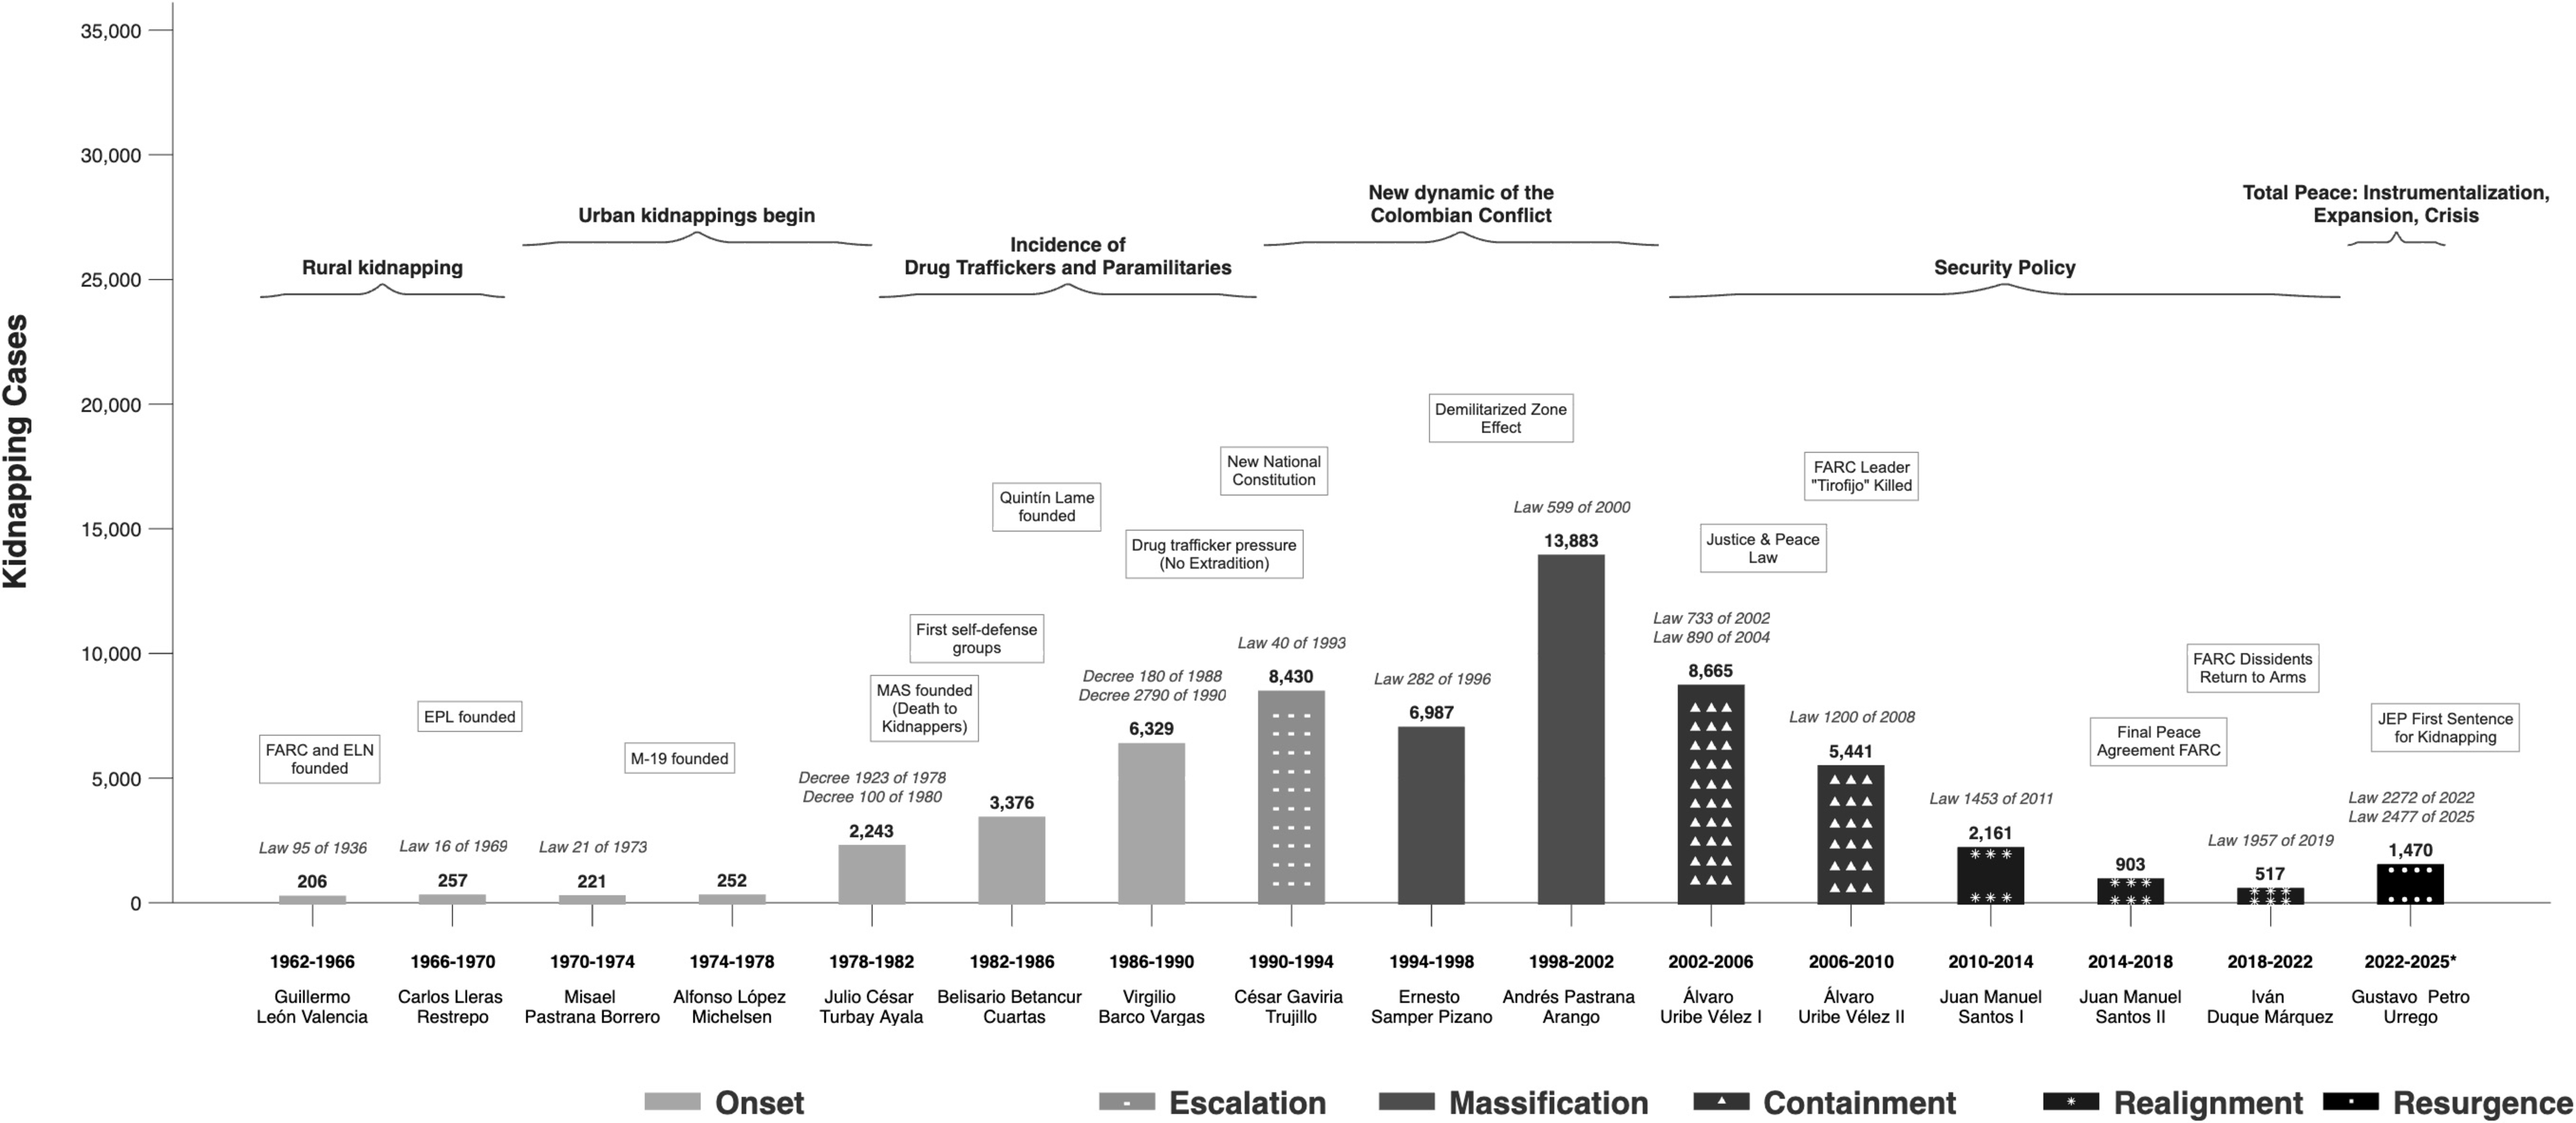
\includegraphics[width=\linewidth]{Fig_4.pdf}
\caption{Evolution of kidnappings in Colombia: armed conflict, security policy, and institutional change (1962--2025).}
\label{fig:evolucion-historica}
\figurenote{\textit{Note:} The figure presents the total number of kidnappings per presidential term in Colombia from 1962 to 2025. Shading distinguishes phases of the armed conflict, and annotations highlight developments related to armed groups, legal reforms, and security policies. \textit{Source:} Author's elaboration based on \citet{cnmh_datos} and \citet{pinto2004}.}
\end{figure}

By estimating two complementary models, a Multinomial Logit (MNL) model and a cause-specific proportional hazards model of \citet{Cox1972}, on $n=1{,}125$ individual-level cases from the National Center for Historical Memory \citep{cnmh_datos}, with full specification, robustness checks, and sample-selection diagnostics detailed in Appendix A, organizational heterogeneity in Colombian kidnapping is quantified. First, static marginal probabilities of outcome are derived from the MNL; specifically, the marginal probability of mortality in captivity ranges from 0.002 for the FARC to 0.071 for common delinquency (DC). Second, cause-specific hazard ratios (HR) are derived from the proportional hazards model of \citet{Cox1972}; estimates show that payment hazard ratios relative to the FARC reach 4.28 for paramilitaries (PAR) and 1.71 for DC, while the ELN is statistically indistinguishable from the reference group; post-2011, the rescue hazard multiplies by 4.86 and the payment hazard falls by 49\%, reflecting the impact of the GAULA's strengthened deterrent and operational capacity. Lastly, temporal profiles of survival, rescue, and mortality are analyzed. Temporal rescue dynamics by duration category and the heterogeneity in captivity duration survival curves by perpetrator are presented in Figure~\ref{fig:cox-a}. In turn, the cumulative probability of tactical rescue by day 100 varies from 0.27 to 0.33 across types, and the dynamic mortality profile in captivity reproduces the same organizational ordering of the MNL with comparable magnitudes of 0.002 to 0.079, as shown in Figure~\ref{fig:cox-b}. These estimates supply the mechanism's type menu $\ThetaK=\{\text{DC},\text{PAR},\text{ELN},\text{FARC}\}$, order the reservation utility of release $U^K_{\mathrm{rel}}(\theta)$ across types, and anchor the type-specific effective intensities $\tilde\lambda_j(t\mid\theta_K)$ whose empirical separation is the observational counterpart of the total-variation separation hypothesis in Lemma~\ref{lem:hazard-separation}.

\begin{figure}[H]
\centering
\captionsetup[subfigure]{justification=centering,singlelinecheck=false}
\begin{subfigure}[t]{0.48\linewidth}
  \centering
  \parbox[t][\subfigheight][b]{\linewidth}{%
    \centering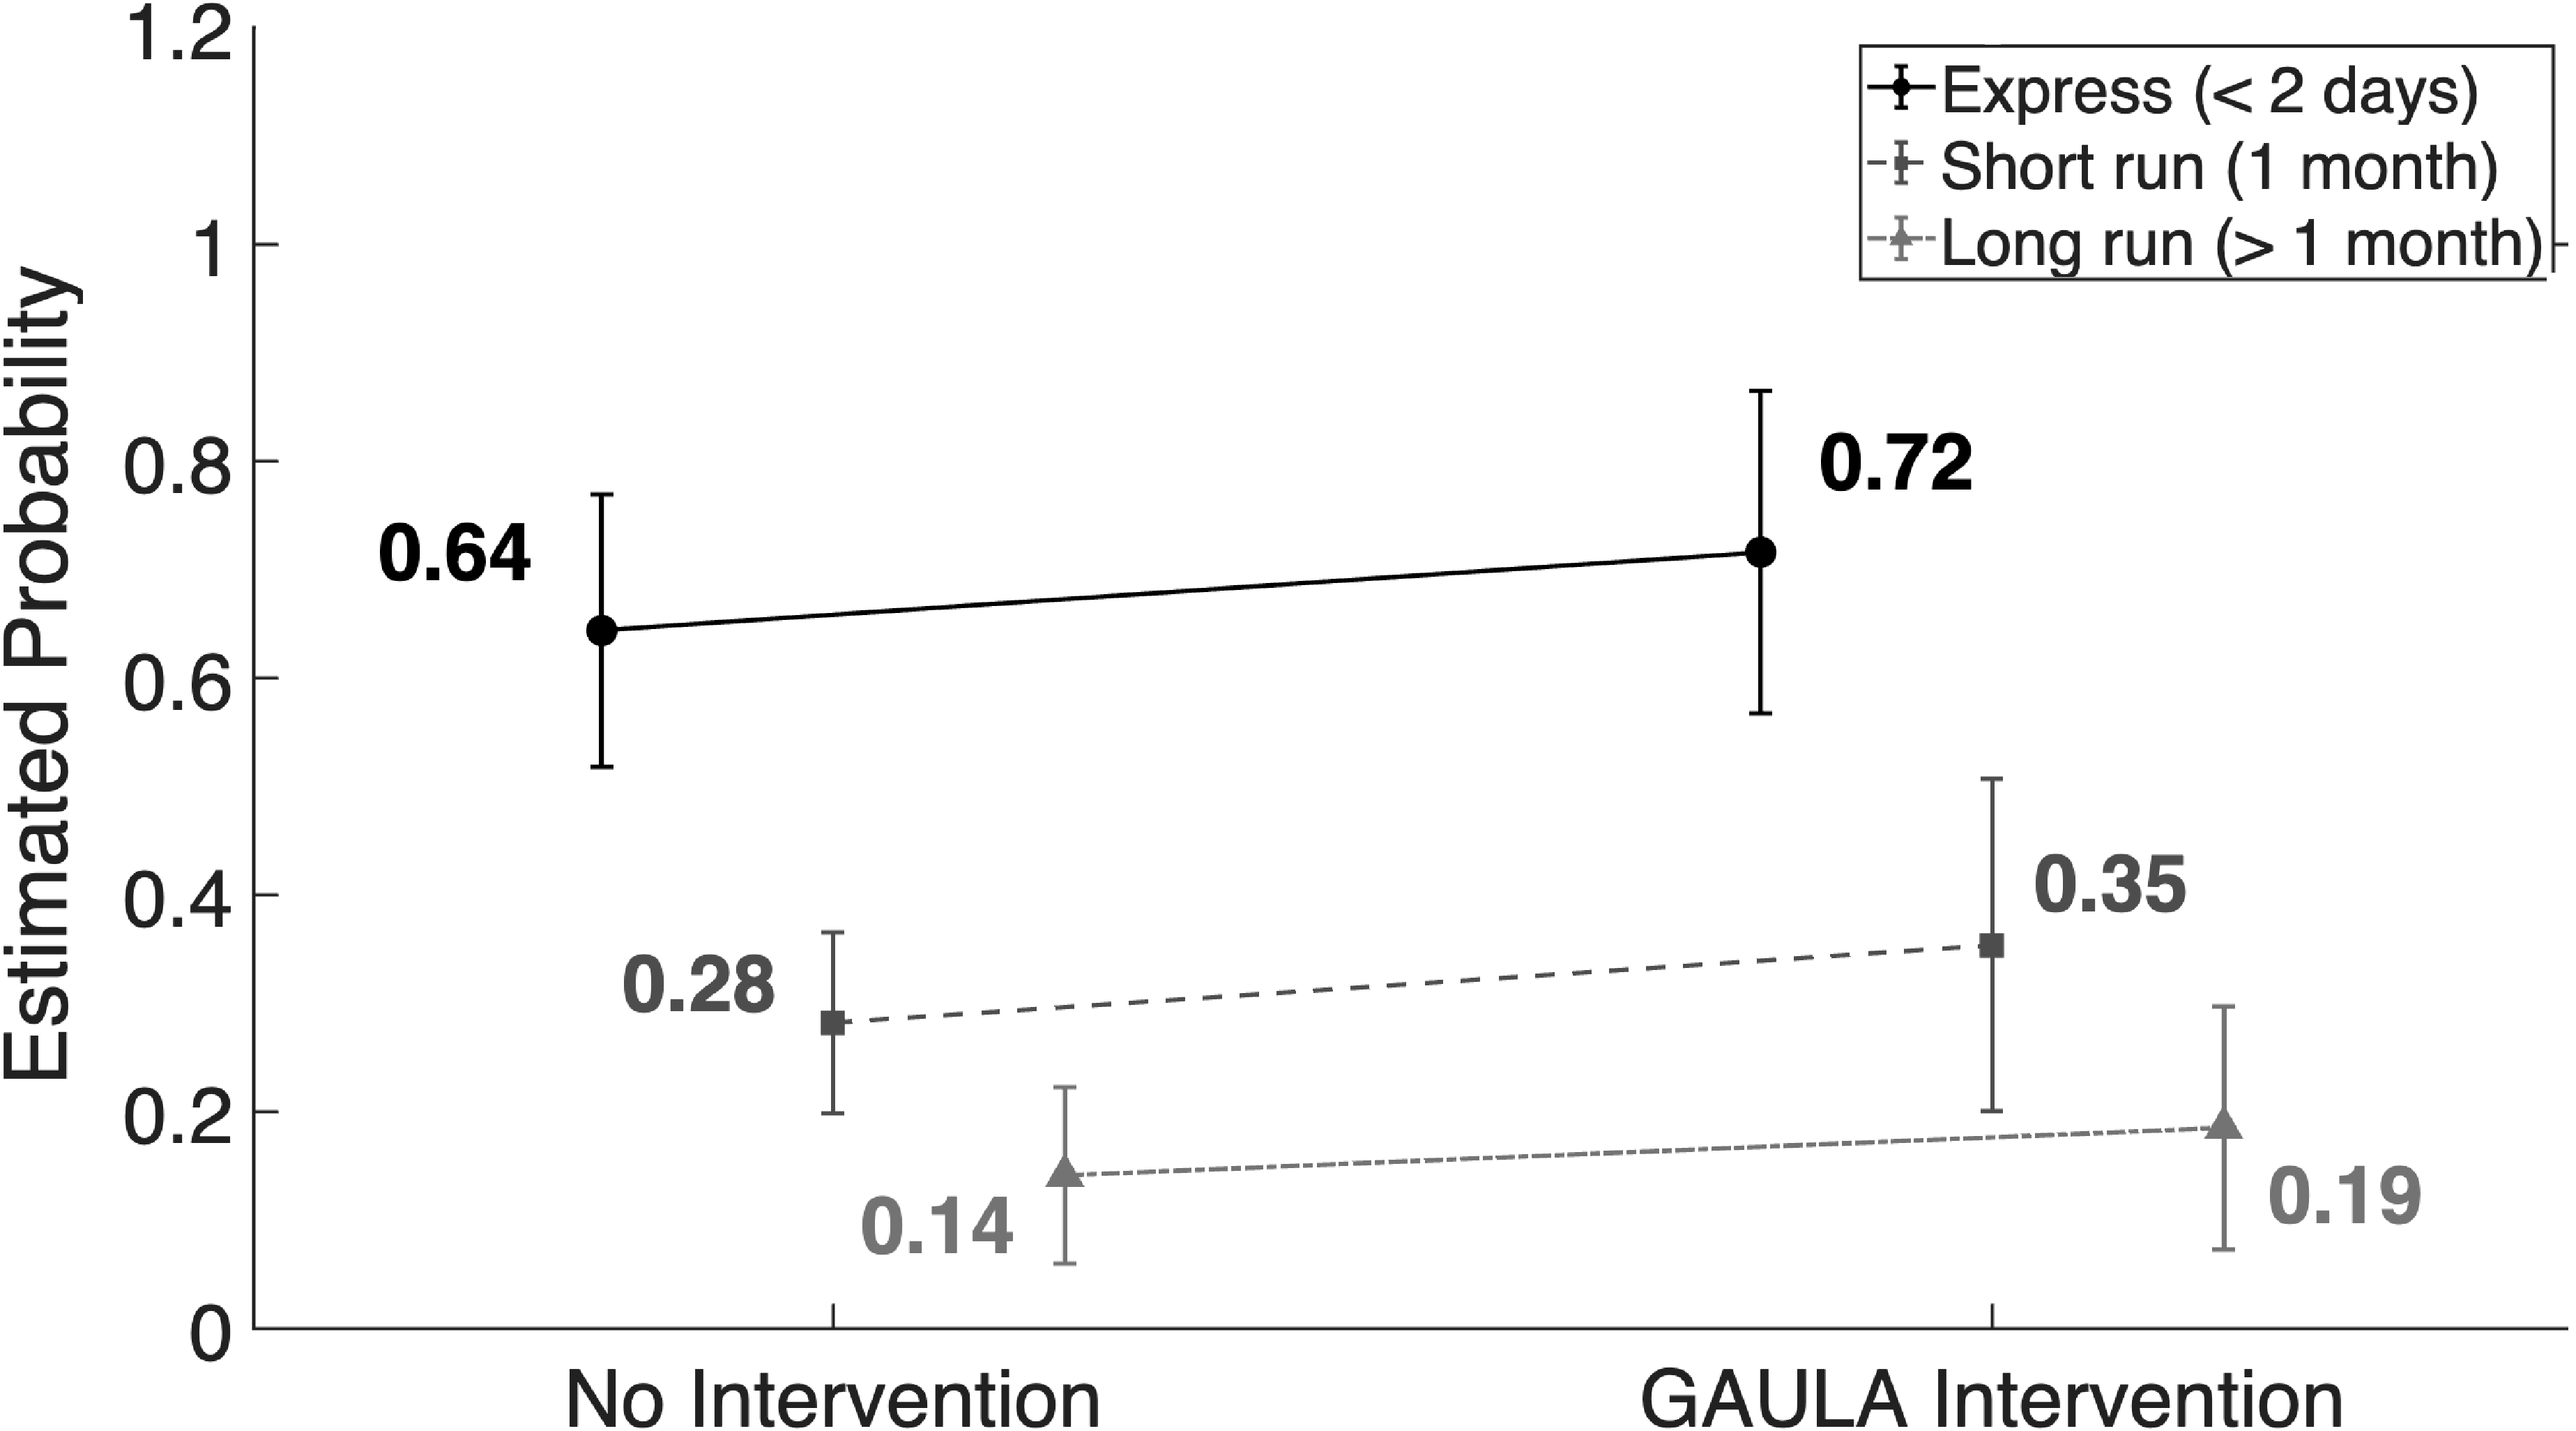
\includegraphics[width=\linewidth,height=\subfigheight,keepaspectratio]{Fig_9a.pdf}%
  }
  \caption{Rescue by GAULA intervention and duration}
\end{subfigure}\hfill
\begin{subfigure}[t]{0.48\linewidth}
  \centering
  \parbox[t][\subfigheight][b]{\linewidth}{%
    \centering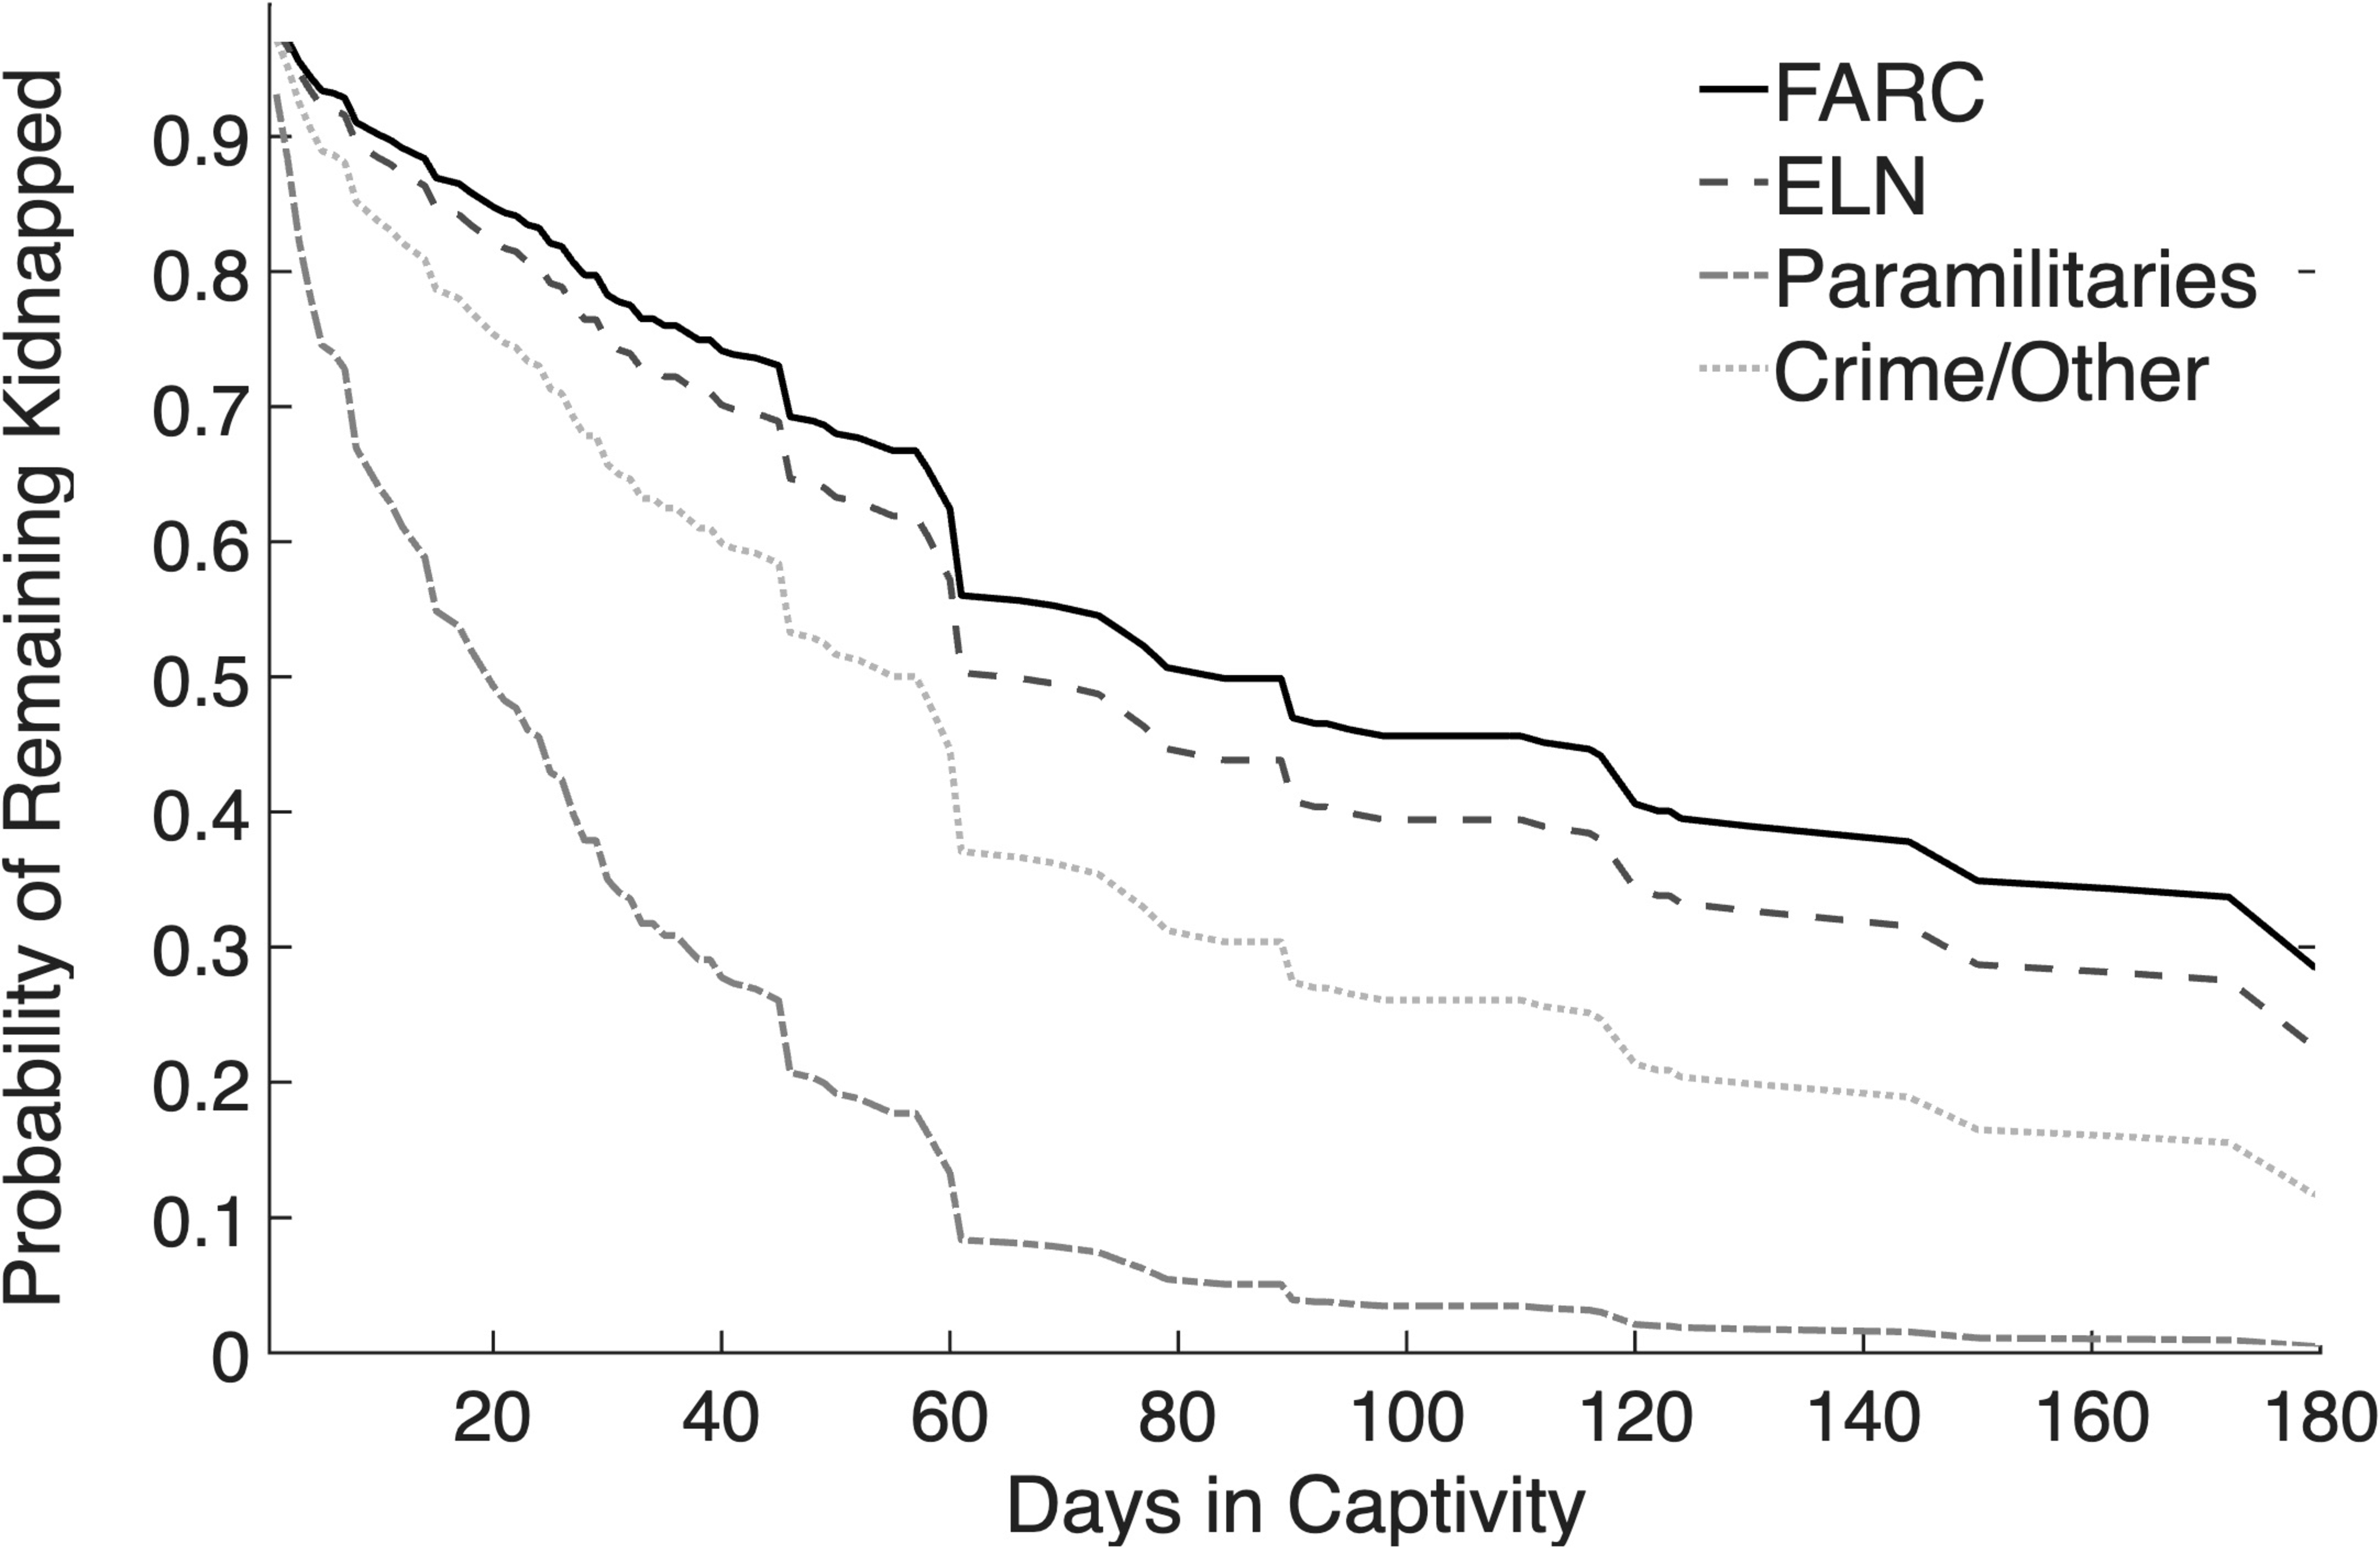
\includegraphics[width=\linewidth,height=\subfigheight,keepaspectratio]{Fig_9b.pdf}%
  }
  \caption{Survival of duration by perpetrator}
\end{subfigure}
\caption{Temporal dynamics of rescue and heterogeneity in captivity duration.}
\label{fig:cox-a}
\figurenote{\textit{Note:} Panel (a) reports the probability of Rescue by GAULA intervention and duration category. Panel (b) presents the survival curves of captivity duration by perpetrator group. \textit{Source:} Author's calculations based on \citet{cnmh_datos}.}
\end{figure}

\begin{figure}[H]
\centering
\begin{subfigure}[t]{0.48\linewidth}
  \centering
  \panelgraphic{\subfigheight}{Fig_10a.pdf}
  \caption{Cumulative state Rescue probability}
\end{subfigure}\hfill
\begin{subfigure}[t]{0.48\linewidth}
  \centering
  \panelgraphic{\subfigheight}{Fig_10b.pdf}
  \caption{Mortality in captivity by perpetrator group}
\end{subfigure}
\caption{Cumulative rescue probability and mortality in captivity by armed group.}
\label{fig:cox-b}
\figurenote{\textit{Note:} Panel (a) shows the cumulative state Rescue probability by armed group, 1964--2025. Panel (b) reports the probability of Death in captivity by perpetrator group. \textit{Source:} Author's calculations based on \citet{cnmh_datos}.}
\end{figure}

\subsection{From estimators to structural inputs}\label{sec:pertinencia}

The MNL and the Cox model connect microeconomic evidence with the initial distribution $\mu_0\in\Delta(\ThetaK)$ and the technology vectors $\beta_{K,j}(\theta_K)$. The MNL provides the static fingerprint of each type by relating perpetrator, victim, context, and tactics to the conditional distribution of outcomes; thus, the initial belief and terminal payments are set with observed weights. The Cox model provides the dynamic dimension: its cause-specific hazards are transferred to the mechanism as rates $\lambda_j(\theta_K,t)$ that govern the daily signal $\zeta_t$, update the posterior $\mu_t$, and determine the speed of learning. The empirical separation of those rates across organizations is the observational basis of Lemma~\ref{lem:hazard-separation} and the criterion of \citet{Kakutani1948}: if the trajectories induced by the types generate sufficiently distinct laws, the posterior can concentrate on the true type. Together, this microeconometric block converts case-level data into priors, costs, hazards, and constraints directly usable by the dynamic mechanism. The explicit translation protocol between estimators and structural parameters is detailed at the beginning of Section~\ref{sec:calibracion}.

\section{Calibration of the mechanism and simulations}\label{sec:calibracion}
\normalfont\normalsize
This section calibrates the specialized mechanism of Section~\ref{sec:application} in four simulated episodes of finite horizon, holding fixed the general architecture of Section~\ref{sec:model}. The exercise combines microeconometric priors and diagnostics to study four objects: the evolution of beliefs $\mu_t(\theta)$, the signals observed by the state, the response of the instruments $(\alpha_t,\gamma_t)$, and compliance with the IR and IC constraints. \emph{Scenario~I} corresponds to DC, with $\theta_K^\ast=\mathrm{DC}$, lax state, high-wealth family, private victim, and Metropolis location; \emph{Scenario~II} corresponds to PAR, with $\theta_K^\ast=\mathrm{PAR}$, strict state, standard-wealth family, public victim, and Caribbean location; \emph{Scenario~III} corresponds to ELN, with $\theta_K^\ast=\mathrm{ELN}$, strict state, high-wealth family, private victim, and Eastern Plains/Jungle location; and \emph{Scenario~IV} corresponds to FARC, with $\theta_K^\ast=\mathrm{FARC}$, lax state, high-wealth family, public victim, and Pacific / Red Zone location. Both are simulated over a fixed horizon $\bar{T}=150$ periods, and optimal policy is computed from the state's minimization of social cost. In the order $(\mathrm{DC},\mathrm{PAR},\mathrm{ELN},\mathrm{FARC})$, the initial priors are $\mu_0^{\mathrm{DC}}=(0.35,0.35,0.15,0.15)$, $\mu_0^{\mathrm{PAR}}=(0.15,0.15,0.25,0.45)$, $\mu_0^{\mathrm{ELN}}=(0.05,0.35,0.25,0.35)$, and $\mu_0^{\mathrm{FARC}}=(0.35,0.35,0.15,0.15)$. In the figures, the gray bar marks the realized stopping time $\tau$; the trajectory after that bar is a counterfactual extension under an absorbing state, following the mechanism law conditioned on non-absorption, that illustrates learning and identification dynamics independently of the closure moment, without constituting a real episode trajectory.

Unlike a purely myopic policy that omits the $-\psi_H\Delta H_t$ term, the calibrated rule in this model internalizes the state's informational subsidy. This allows it to strategically reallocate the $(\alpha_t,\gamma_t)$ instruments toward regions of the grid that maximize the separation of the likelihoods of rival types. As a result, the numerical exercises for the DC, PAR, ELN, and FARC cases illustrate three fundamental operational implications of the theory: first, the concentration of the posterior belief in a finite horizon in the direction predicted by Theorem~\ref{thm:posterior-consistency}; second, the Bayesian updating with full support along the path enabled by the MDG; and third, the ex-post compliance with the $IC^K$, $IR^K$, and $IR^F$ constraints according to the implementability logic described in Theorem~\ref{thm:ebp-implementabilidad}. It is worth emphasizing that these simulations illustrate finite-horizon learning and do not claim to demonstrate asymptotic identification over $\mathcal{T}$, which remains strictly a theoretical limit result.


\begin{figure}[H]
\centering
\begin{subfigure}[t]{0.48\linewidth}
  \centering
  \panelgraphic{\calbeliefheight}{Fig_11a.pdf}
  \caption{Scenario I: DC}
\end{subfigure}\hfill
\begin{subfigure}[t]{0.48\linewidth}
  \centering
  \panelgraphic{\calbeliefheight}{Fig_11b.pdf}
  \caption{Scenario II: PAR}
\end{subfigure}

\medskip
\begin{subfigure}[t]{0.48\linewidth}
  \centering
  \panelgraphic{\calbeliefheight}{Fig_11c.pdf}
  \caption{Scenario III: ELN}
\end{subfigure}\hfill
\begin{subfigure}[t]{0.48\linewidth}
  \centering
  \panelgraphic{\calbeliefheight}{Fig_11d.pdf}
  \caption{Scenario IV: FARC}
\end{subfigure}
\caption{Bayesian beliefs of each type $\mu_\tau(\theta)$ across scenarios.}
\label{fig:cal-eln-par-mu}
\figurenote{\textit{Note:} Panel (a) corresponds to Scenario~I: $\theta_K^\ast=\mathrm{DC}$, lax $\theta_S$, high-wealth $\theta_F$, private $\theta_V$, and Metropolis $z$. Panel (b) corresponds to Scenario~II: $\theta_K^\ast=\mathrm{PAR}$, strict $\theta_S$, standard-wealth $\theta_F$, public $\theta_V$, and Caribbean $z$. Panel (c) corresponds to Scenario~III: $\theta_K^\ast=\mathrm{ELN}$, strict $\theta_S$, high-wealth $\theta_F$, private $\theta_V$, and Eastern Plains/Jungle $z$. Panel (d) corresponds to Scenario~IV: $\theta_K^\ast=\mathrm{FARC}$, lax $\theta_S$, high-wealth $\theta_F$, public $\theta_V$, and Pacific / Red Zone $z$. The gray band marks $\tau^{\mathrm{hyp}}$, the first period in which the mechanism outcome differs from continuation.}
\end{figure}
\vspace{-8pt}
The posterior of the true type allows evaluating the capability of the mechanism to separate types from the sequence of signals. As reported in Figure~\ref{fig:cal-eln-par-mu}, posterior mass shifts gradually toward the true type in all four scenarios, reaching $\mu_{150}(\theta_K^\ast)\approx 1{,}000$; this implies that the mechanism accumulates identification across different wealth levels, locations, and victim sectors. In Scenario~I and Scenario~IV, the posterior concentration is rapid. In Scenario~II and Scenario~III, the trajectories are less monotonic in the initial phase, reflecting early signals compatible with alternative types before eventually shifting mass toward the true perpetrator. The gray bars mark the realized stopping times; the subsequent counterfactual extensions show that the speed of learning and the absorption moment are distinct objects of the model. Taken together, the figure illustrates finite-horizon behavior: posterior mass shifts toward the true type as signals accumulate separation, in the direction predicted by Theorem~\ref{thm:posterior-consistency} under $\mathcal{T}$, without constituting direct evidence for the asymptotic result; the speed of convergence depends on the institutional, territorial, and case-visibility environment.

\begin{figure}[H]
\centering
\begin{subfigure}[t]{0.48\linewidth}
  \centering
  \panelgraphic{\calseriesheight}{Fig_12a.pdf}
  \caption{Scenario I: DC}
\end{subfigure}\hfill
\begin{subfigure}[t]{0.48\linewidth}
  \centering
  \panelgraphic{\calseriesheight}{Fig_12b.pdf}
  \caption{Scenario II: PAR}
\end{subfigure}

\medskip
\begin{subfigure}[t]{0.48\linewidth}
  \centering
  \panelgraphic{\calseriesheight}{Fig_12c.pdf}
  \caption{Scenario III: ELN}
\end{subfigure}\hfill
\begin{subfigure}[t]{0.48\linewidth}
  \centering
  \panelgraphic{\calseriesheight}{Fig_12d.pdf}
  \caption{Scenario IV: FARC}
\end{subfigure}
\caption{Operational pressure $\gamma_t^\ast$ and benchmark $\gamma^R$ against $\tau$.}
\label{fig:cal-eln-par-gamma}
\figurenote{\textit{Note:} Panel (a) shows the operational pressure trajectory in Scenario~I (DC). Panel (b) shows the equivalent trajectory in Scenario~II (PAR). Panel (c) shows Scenario~III (ELN). Panel (d) shows Scenario~IV (FARC). The dashed line corresponds to the Rescue benchmark $\gamma^R$. The gray band marks $\tau^{\mathrm{hyp}}$.}
\end{figure}
The optimal operational pressure allows evaluating how the state adjusts the intensity of intervention as it learns about the captor's type. Figure~\ref{fig:cal-eln-par-gamma} compares the trajectory of $\gamma_t^\ast$ with the Rescue benchmark $\gamma^R$, which takes the value $\gamma^R=0{,}23$ in DC, $\gamma^R=0{,}37$ in PAR, $\gamma^R=0{,}50$ in ELN, and $\gamma^R=0{,}64$ in FARC. In Scenario~I (DC), $\gamma_t^\ast$ is located on average around $\bar\gamma^\ast\approx 0{,}564$. In Scenario~II (PAR), pressure reaches $\bar\gamma^\ast\approx 0{,}662$. In Scenario~III (ELN), average pressure is $\bar\gamma^\ast\approx 0{,}663$, and in Scenario~IV (FARC), it is $\bar\gamma^\ast\approx 0{,}715$. In all cases, $\gamma_t^\ast$ does not mechanically replicate either the Rescue or the Negotiate branch: dual control combines exploitation of the instrument and expected information, so the series fluctuates between benchmarks according to the material risk of the episode and the value of separating types.

The optimal financial interdiction summarizes the intensity with which the state restricts payment capacity and economic coordination during the episode. Figure~\ref{fig:cal-eln-par-alpha} compares the trajectory of $\alpha_t^\ast$ with the Rescue benchmark $\alpha^R$, which takes the value $\alpha^R=0{,}18$ in DC, $\alpha^R=0{,}31$ in PAR, $\alpha^R=0{,}45$ in ELN, and $\alpha^R=0{,}59$ in FARC. In Scenario~I (DC), $\bar\alpha^\ast\approx 0{,}896$. In Scenario~II (PAR), $\bar\alpha^\ast\approx 0{,}730$. In Scenario~III (ELN), $\bar\alpha^\ast\approx 0{,}737$, and in Scenario~IV (FARC), $\bar\alpha^\ast\approx 0{,}755$. Thus, $\alpha_t^\ast$ does not mechanically replicate a pure branch: it moves between Rescue and Negotiate benchmarks according to accumulated information, family payment capacity, and the value of inducing separation among types.

The posterior precision, defined as $\iota_t=\max_{\theta\in\ThetaK}\mu_t(\theta)$, allows observing how operational pressure changes when the state gains confidence about the identity of the true type. Figure~\ref{fig:cal-eln-par-iota-gamma} reorders the simulation on the plane $(\iota_t,\gamma_t^\ast)$; the arrows indicate the advance of $\tau$ and avoid interpreting the observations as a linear interpolation. The trajectory concentrates in zones of high pressure and rising precision, reflecting learning without immediate collapse toward a single dominant signal, and showcasing the distinct dynamics across cases.
\vspace{-4pt}
\begin{figure}[H]
\centering
\begin{subfigure}[t]{0.48\linewidth}
  \centering
  \panelgraphic{\calseriesheight}{Fig_13a.pdf}
  \caption{Scenario I: DC}
\end{subfigure}\hfill
\begin{subfigure}[t]{0.48\linewidth}
  \centering
  \panelgraphic{\calseriesheight}{Fig_13b.pdf}
  \caption{Scenario II: PAR}
\end{subfigure}

\medskip
\begin{subfigure}[t]{0.48\linewidth}
  \centering
  \panelgraphic{\calseriesheight}{Fig_13c.pdf}
  \caption{Scenario III: ELN}
\end{subfigure}\hfill
\begin{subfigure}[t]{0.48\linewidth}
  \centering
  \panelgraphic{\calseriesheight}{Fig_13d.pdf}
  \caption{Scenario IV: FARC}
\end{subfigure}
\caption{Financial interdiction $\alpha_t^\ast$ and benchmark $\alpha^R$ against $\tau$.}
\label{fig:cal-eln-par-alpha}
\figurenote{\textit{Note:} Panel (a) presents the optimal financial interdiction in Scenario~I (DC). Panel (b) presents Scenario~II (PAR). Panel (c) presents Scenario~III (ELN). Panel (d) presents Scenario~IV (FARC). The dashed line corresponds to the Rescue benchmark $\alpha^R$. The gray band marks $\tau^{\mathrm{hyp}}$.}
\end{figure}
\vspace{-6pt}
Financial interdiction against posterior precision allows evaluating whether learning reduces or reinforces the need to restrict payment capacity. As reported in Figure~\ref{fig:cal-eln-par-iota-alpha}, $\alpha_t^\ast$ remains high while $\iota_t$ increases across all scenarios, indicating that identifying the true type does not eliminate the value of maintaining preventive interdiction. This pattern is consistent with environments where financial interdiction retains relevance as an instrument of control, payment containment, and induction of separation among types.
\vspace{-4pt}
\begin{figure}[H]
\centering
\begin{subfigure}[t]{0.48\linewidth}
  \centering
  \panelgraphic{\calfigheight}{Fig_14a.pdf}
  \caption{Scenario I: DC}
\end{subfigure}\hfill
\begin{subfigure}[t]{0.48\linewidth}
  \centering
  \panelgraphic{\calfigheight}{Fig_14b.pdf}
  \caption{Scenario II: PAR}
\end{subfigure}

\medskip
\begin{subfigure}[t]{0.48\linewidth}
  \centering
  \panelgraphic{\calfigheight}{Fig_14c.pdf}
  \caption{Scenario III: ELN}
\end{subfigure}\hfill
\begin{subfigure}[t]{0.48\linewidth}
  \centering
  \panelgraphic{\calfigheight}{Fig_14d.pdf}
  \caption{Scenario IV: FARC}
\end{subfigure}
\caption{Trajectory $(\iota_t,\gamma_t^\ast)$ with arrows indicating temporal advance.}
\label{fig:cal-eln-par-iota-gamma}
\figurenote{\textit{Note:} Panel (a) corresponds to Scenario~I (DC), panel (b) to Scenario~II (PAR), panel (c) to Scenario~III (ELN), and panel (d) to Scenario~IV (FARC). Each trajectory shows 20 arrows indicating direction; the circle identifies the end point, $\tau=150$.}
\end{figure}
\vspace{-6pt}
The constraints diagnostic confirms that the strategic feasibility of the mechanism is preserved across all scenarios. As Figure~\ref{fig:cal-eln-par-iric} shows, the captor's incentive constraint ($\mathrm{IC}^K$), the captor's participation constraint ($\mathrm{IR}^K$), and the family's participation constraint ($\mathrm{IR}^F$) are satisfied in all 150 simulated cycles in all four scenarios. The verification is \emph{a posteriori} with respect to the true type $\theta_K^\ast$: the optimal instruments $(a_S^\ast,\alpha_t^\ast,\gamma_t^\ast)$ are evaluated directly on the utilities of the true type, without weighting by the belief $\mu_t$. The mechanism is therefore feasible in an ex-post sense: given $\theta_K^\ast$, optimal policy satisfies incentive compatibility and participation without abandoning the informational component.
\vspace{-4pt}
\begin{figure}[H]
\centering
\begin{subfigure}[t]{0.48\linewidth}
  \centering
  \panelgraphic{\calfigheight}{Fig_15a.pdf}
  \caption{Scenario I: DC}
\end{subfigure}\hfill
\begin{subfigure}[t]{0.48\linewidth}
  \centering
  \panelgraphic{\calfigheight}{Fig_15b.pdf}
  \caption{Scenario II: PAR}
\end{subfigure}

\medskip
\begin{subfigure}[t]{0.48\linewidth}
  \centering
  \panelgraphic{\calfigheight}{Fig_15c.pdf}
  \caption{Scenario III: ELN}
\end{subfigure}\hfill
\begin{subfigure}[t]{0.48\linewidth}
  \centering
  \panelgraphic{\calfigheight}{Fig_15d.pdf}
  \caption{Scenario IV: FARC}
\end{subfigure}
\caption{Trajectory $(\iota_t,\alpha_t^\ast)$ with arrows indicating temporal advance.}
\label{fig:cal-eln-par-iota-alpha}
\figurenote{\textit{Note:} Panel (a) corresponds to Scenario~I (DC), panel (b) to Scenario~II (PAR), panel (c) to Scenario~III (ELN), and panel (d) to Scenario~IV (FARC). Each trajectory shows 20 arrows indicating direction; the circle identifies the end point, $\tau=150$.}
\end{figure}
\clearpage
\begin{figure}[H]
\centering
\begin{subfigure}[t]{0.48\linewidth}
  \centering
  \panelgraphic{\calfigheight}{Fig_16a.pdf}
  \caption{Scenario I: DC}
\end{subfigure}\hfill
\begin{subfigure}[t]{0.48\linewidth}
  \centering
  \panelgraphic{\calfigheight}{Fig_16b.pdf}
  \caption{Scenario II: PAR}
\end{subfigure}

\medskip
\begin{subfigure}[t]{0.48\linewidth}
  \centering
  \panelgraphic{\calfigheight}{Fig_16c.pdf}
  \caption{Scenario III: ELN}
\end{subfigure}\hfill
\begin{subfigure}[t]{0.48\linewidth}
  \centering
  \panelgraphic{\calfigheight}{Fig_16d.pdf}
  \caption{Scenario IV: FARC}
\end{subfigure}
\caption{Frequency of compliance with $\mathrm{IC}^K$, $\mathrm{IR}^K$, and $\mathrm{IR}^F$ (\% of cycles).}
\label{fig:cal-eln-par-iric}
\figurenote{\textit{Note:} Panel (a) summarizes compliance in Scenario~I (DC), panel (b) in Scenario~II (PAR), panel (c) in Scenario~III (ELN), and panel (d) in Scenario~IV (FARC). Percentages are computed over the simulated cycles of each scenario.}
\end{figure}
\vspace{-6pt}
The expected informational gain $\Delta H_t$ quantifies the anticipated reduction in entropy induced by the state's instruments, in the sense of the optimal dynamic acquisition of information of \citet{Zhong2022}. That informational subsidy concentrates at the start of the simulation, as illustrated in Figure~\ref{fig:cal-eln-par-dh}: in DC it reaches its maximum at $\tau=10$ with $\Delta H_{10}\approx 0{,}043$, and in PAR at $\tau=6$ with $\Delta H_6\approx 0{,}035$. As $\Delta H_t$ converges to zero, additional observations cease to reduce posterior uncertainty and optimal decision comes to be governed by material losses and a belief already concentrated on the true type.
\vspace{-4pt}
\begin{figure}[H]
\centering
\begin{subfigure}[t]{0.48\linewidth}
  \centering
  \panelgraphic{\calfigheight}{Fig_17a.pdf}
  \caption{Scenario I: DC}
\end{subfigure}\hfill
\begin{subfigure}[t]{0.48\linewidth}
  \centering
  \panelgraphic{\calfigheight}{Fig_17b.pdf}
  \caption{Scenario II: PAR}
\end{subfigure}

\medskip
\begin{subfigure}[t]{0.48\linewidth}
  \centering
  \panelgraphic{\calfigheight}{Fig_17c.pdf}
  \caption{Scenario III: ELN}
\end{subfigure}\hfill
\begin{subfigure}[t]{0.48\linewidth}
  \centering
  \panelgraphic{\calfigheight}{Fig_17d.pdf}
  \caption{Scenario IV: FARC}
\end{subfigure}
\caption{Expected informational gain $\Delta H_t$ against $\tau$.}
\label{fig:cal-eln-par-dh}
\figurenote{\textit{Note:} Panel (a) corresponds to Scenario~I (DC), panel (b) to Scenario~II (PAR), panel (c) to Scenario~III (ELN), and panel (d) to Scenario~IV (FARC). The series reports expected entropy reduction in each simulated cycle.}
\end{figure}
\vspace{-6pt}
In all scenarios and for all types, $\kappa_h(\theta_K^\ast,t)>0$ in 100\,\% of simulated cycles, as shown in Figure~\ref{fig:cal-eln-par-kh}. By the relation $\operatorname{sgn}(\partial\,\mathbb{E}[\tau\mid\theta_K]/\partial\gamma_t^\ast)=-\operatorname{sgn}(\kappa_h)$, this implies $\partial\,\mathbb{E}[\tau\mid\theta_K]/\partial\gamma_t^\ast<0$: higher operational pressure \emph{reduces} expected captivity duration without exception. The mechanism does not face a trade-off between exploiting the instrument and learning: operational pressure shortens captivity and, by modifying closure hazards, simultaneously generates signals that separate the likelihoods of rival types and accelerate posterior convergence.
\vspace{-4pt}
\begin{figure}[H]
\centering
\begin{subfigure}[t]{0.48\linewidth}
  \centering
  \panelgraphic{\calseriesheight}{Fig_18a.pdf}
  \caption{Scenario I: DC}
\end{subfigure}\hfill
\begin{subfigure}[t]{0.48\linewidth}
  \centering
  \panelgraphic{\calseriesheight}{Fig_18b.pdf}
  \caption{Scenario II: PAR}
\end{subfigure}

\medskip
\begin{subfigure}[t]{0.48\linewidth}
  \centering
  \panelgraphic{\calseriesheight}{Fig_18c.pdf}
  \caption{Scenario III: ELN}
\end{subfigure}\hfill
\begin{subfigure}[t]{0.48\linewidth}
  \centering
  \panelgraphic{\calseriesheight}{Fig_18d.pdf}
  \caption{Scenario IV: FARC}
\end{subfigure}
\caption{Net sensitivity $\kappa_h(\theta_K^\ast,t)$ of expected captivity duration with respect to $\gamma_t^\ast$.}
\label{fig:cal-eln-par-kh}
\figurenote{\textit{Note:} Each panel traces $\kappa_h(\theta_K^\ast,t)$ for the true type of the scenario. A constant value of $+1$ implies $-\operatorname{sgn}(\kappa_h)=-1$ in 100\,\% of cycles, that is, $\partial\,\mathbb{E}[\tau\mid\theta_K]/\partial\gamma_t^\ast<0$; the horizontal dashed line marks the reference zero.}
\end{figure}
\vspace{-6pt}
The hypothetical terminal outcomes differ across scenarios: \emph{Ransom Paid} in DC ($\tau^{\mathrm{hyp}}=35$), \emph{Rescue} in PAR ($\tau^{\mathrm{hyp}}=105$), \emph{Release} in ELN ($\tau^{\mathrm{hyp}}=75$), and \emph{Rescue} in FARC ($\tau^{\mathrm{hyp}}=20$). In all cases the posterior starts from its initial prior and converges to $\mu_{150}(\theta^\ast)\approx 1{,}000$, with $\bar\alpha^\ast$ and $\bar\gamma^\ast$ above 0{,}56 in all scenarios. These results are summarized in Table~\ref{tab:calibracion-resumen}.

\begin{table}[htbp]
\centering
\caption{Summary of dynamic calibration by scenario}
\label{tab:calibracion-resumen}
\small
\begin{tabular}{lrrrrrl}
\toprule
$\theta_K^\ast$ & $\mu_0(\theta^\ast)$ & $\mu_{\tau_{\max}}(\theta^\ast)$ & $\bar{\alpha}^\ast$ & $\bar{\gamma}^\ast$ & $\tau^{\mathrm{hyp}}$ & $m_{\tau^{\mathrm{hyp}}}$ \\
\midrule
DC & 0.350 & 1.000 & 0.896 & 0.564 & 35 & Ransom Paid \\
PAR & 0.150 & 1.000 & 0.730 & 0.662 & 105 & Rescue \\
ELN & 0.250 & 1.000 & 0.737 & 0.663 & 75 & Release \\
FARC & 0.150 & 1.000 & 0.755 & 0.715 & 20 & Rescue \\
\bottomrule
\end{tabular}
\end{table}

Taken together, the ELN--PAR contrast shows that the same Bayesian mechanism generates distinct learning trajectories, instrument intensities, and constraint viability rates when, jointly, the captor's true type and the institutional, family, victim, and geographic margins described in the protocol change. The simulations do not substitute for Theorem~\ref{thm:posterior-consistency}, which requires recurrent separation in the event $\mathcal{T}$; they illustrate that, with priors and hazards calibrated to Colombian evidence, the entropic subsidy shifts policy away from purely myopic regimes and accelerates or disciplines posterior concentration in finite horizons, in the direction predicted by the identification result.

\section{Discussion and conclusions}\label{sec:conclusiones}

This paper develops an indirect dynamic mechanism for environments in which equilibrium actions pool and types are not elicited by free reports. Relative to the classical reduction via the Revelation Principle, the contribution is to construct the operational indirect object: public instruments, endogenous implementation noise, and Bayesian learning over action-generated signals.

At the theoretical level, the MDG kernel supplies full-support materialization of latent intentions without an exogenous tremble, keeping Bayes' rule well defined off path. The Type Identification Theorem shows that recurrent total-variation separation of type-contingent observation laws implies mutual singularity of trajectory measures and almost-sure posterior concentration on the true type on the prolonged-interaction event $\mathcal{T}$. The Conditional Implementability Theorem complements identification by guaranteeing a PBE that satisfies incentive compatibility and individual rationality whenever the feasible set remains non-empty. The asymptotic result is intentionally sharp: it clarifies the informational limit of the architecture; finite-horizon behavior is a distinct, applied object.

At the applied level, Colombian kidnapping for ransom maps the abstract type space into estimated criminal technologies. Competing-risks and multinomial evidence discipline hazards and priors; ELN--PAR simulations show that the calibrated dual-control rule accelerates posterior concentration, sustains high but disciplined instruments, and preserves IR/IC feasibility, in the direction predicted by the theorems without substituting for them.

Two extensions are natural. The first is a finite-horizon identification bound that translates total-variation separation into explicit posterior concentration rates under endogenous stopping. The second is multi-agent concurrent identification when several privately informed parties interact under a shared public history. Both would transfer the framework beyond adversarial screening to other markets with noisy implementation and observational pooling.


\section*{Declaration on the use of Generative Artificial Intelligence}

In the preparation of this manuscript, the author used generative artificial intelligence tools, specifically \emph{Cursor} and \emph{Antigravity}, to assist in the following tasks: literature review and text editing; programming in Lean 4 for the formalization and interactive proof of theoretical theorems and lemmas; programming of quantitative and empirical code in Matlab, Stata, and Python; as well as the design and online deployment of the calibrated dynamic model interface via GitHub and Streamlit. Consistent with academic ethical guidelines, the author is solely responsible for the integrity of the document, having thoroughly verified and validated all information, proofs, estimations, and codes provided or generated by these technologies.

\bibliographystyle{econsoc}

\bibliography{references}

\end{document}
